\documentclass[handout,compress]{beamer}

\usetheme[block=fill]{metropolis}

\usepackage{graphicx} % Allows including images
\usepackage{amsmath,amsfonts,amsthm,amssymb}
\usepackage{color}
\usepackage{xcolor,cancel}
%\setitemize{label=\usebeamerfont*{itemize item}%
%	\usebeamercolor[fg]{itemize item}
%	\usebeamertemplate{itemize item}}
\definecolor{mDarkBrown}{HTML}{604c38}
\definecolor{mDarkTeal}{HTML}{23373b}
\definecolor{mLightBrown}{HTML}{EB811B}
\definecolor{mMediumBrown}{HTML}{C87A2F}
\definecolor{mygreen}{HTML}{98C2B9}
\definecolor{myyellow}{HTML}{DFD79C}
\definecolor{myblue}{HTML}{8CA7CC}
\definecolor{kern}{HTML}{8CC2B7}

\usepackage{float}
\usepackage{framed}
\usepackage{epsfig}
\usepackage{graphicx}
\usepackage{subcaption}
\usepackage{ulem}
\usepackage{hhline}
\usepackage{multirow}
\usepackage{comment}   
\usepackage{bbm}
\usepackage{tikz}   
\usepackage{ulem}
\def\Put(#1,#2)#3{\leavevmode\makebox(0,0){\put(#1,#2){#3}}}
\newcommand*\mystrut[1]{\vrule width0pt height0pt depth#1\relax}
\newcommand{\eqdef}{\mathbin{\stackrel{\rm def}{=}}}


\newcommand{\bs}[1]{\boldsymbol{#1}}
\newcommand{\bv}[1]{\mathbf{#1}}
\newcommand{\R}{\mathbb{R}}
\newcommand{\E}{\mathbb{E}}

\DeclareMathOperator*{\argmin}{arg\,min}
\DeclareMathOperator*{\argmax}{arg\,max}
\DeclareMathOperator{\nnz}{nnz}
\DeclareMathOperator{\Var}{Var}
\DeclareMathOperator{\sinc}{sinc}
\DeclareMathOperator{\mv}{mv}
\DeclareMathOperator{\sgn}{sgn}
\DeclareMathOperator{\step}{step}
\DeclareMathOperator{\gap}{gap}
\DeclareMathOperator{\poly}{poly}
\DeclareMathOperator{\tr}{tr}
\DeclareMathOperator{\orth}{orth}
\newcommand{\norm}[1]{\|#1\|}
\captionsetup[subfigure]{labelformat=empty}
\captionsetup[figure]{labelformat=empty}
\DeclareMathOperator*{\lmin}{\lambda_{min}}
\DeclareMathOperator*{\lmax}{\lambda_{max}}

\newcommand{\specialcell}[2][c]{%
	\begin{tabular}[#1]{@{}c@{}}#2\end{tabular}}
\newcommand{\specialcellleft}[2][c]{%
	\begin{tabular}[#1]{@{}l@{}}#2\end{tabular}
}

\usepackage{tabstackengine}
\stackMath

\newtheorem{claim}[theorem]{Claim}


%----------------------------------------------------------------------------------------
%	TITLE PAGE
%----------------------------------------------------------------------------------------

\title{CS-UY 4563: Lecture 18 \\ Convolutional Feature Extraction}
\author{NYU Tandon School of Engineering, Prof. Christopher Musco}
\date{}

\begin{document}
	
	\begin{frame}
		\titlepage 
	\end{frame}
	
	\metroset{titleformat=smallcaps}
	
	\begin{frame}
		\frametitle{course logistics}
		\begin{itemize}
			\item Midterm 2 exam \textbf{is canceled.}
			\begin{itemize}
				\item In place of midterm grade, you will be awarded maximum grade from your homework, first midterm, or project.  
			\end{itemize}  	
			\item Project Proposal due \textbf{tonight}. 
			\begin{itemize}
				\item See guidelines for what to include at: \url{https://www.chrismusco.com/introml/project_guidelines.pdf}
			\end{itemize} 
			\item New written homework posted. Due \textbf{next Monday}. 
		\end{itemize}
	\end{frame}
	
	\begin{frame}
		\frametitle{neural network demos}
		\textbf{Quick note from last class.} Two demos uploaded on neural networks:
		\begin{itemize}
			\item \texttt{keras\_demo\_synthetic.ipynb}
			\item \texttt{keras\_demo\_mnist.ipynb}
		\end{itemize}
	\end{frame}

	\begin{frame}
	\frametitle{neural network software}
	\small
	\begin{center}
		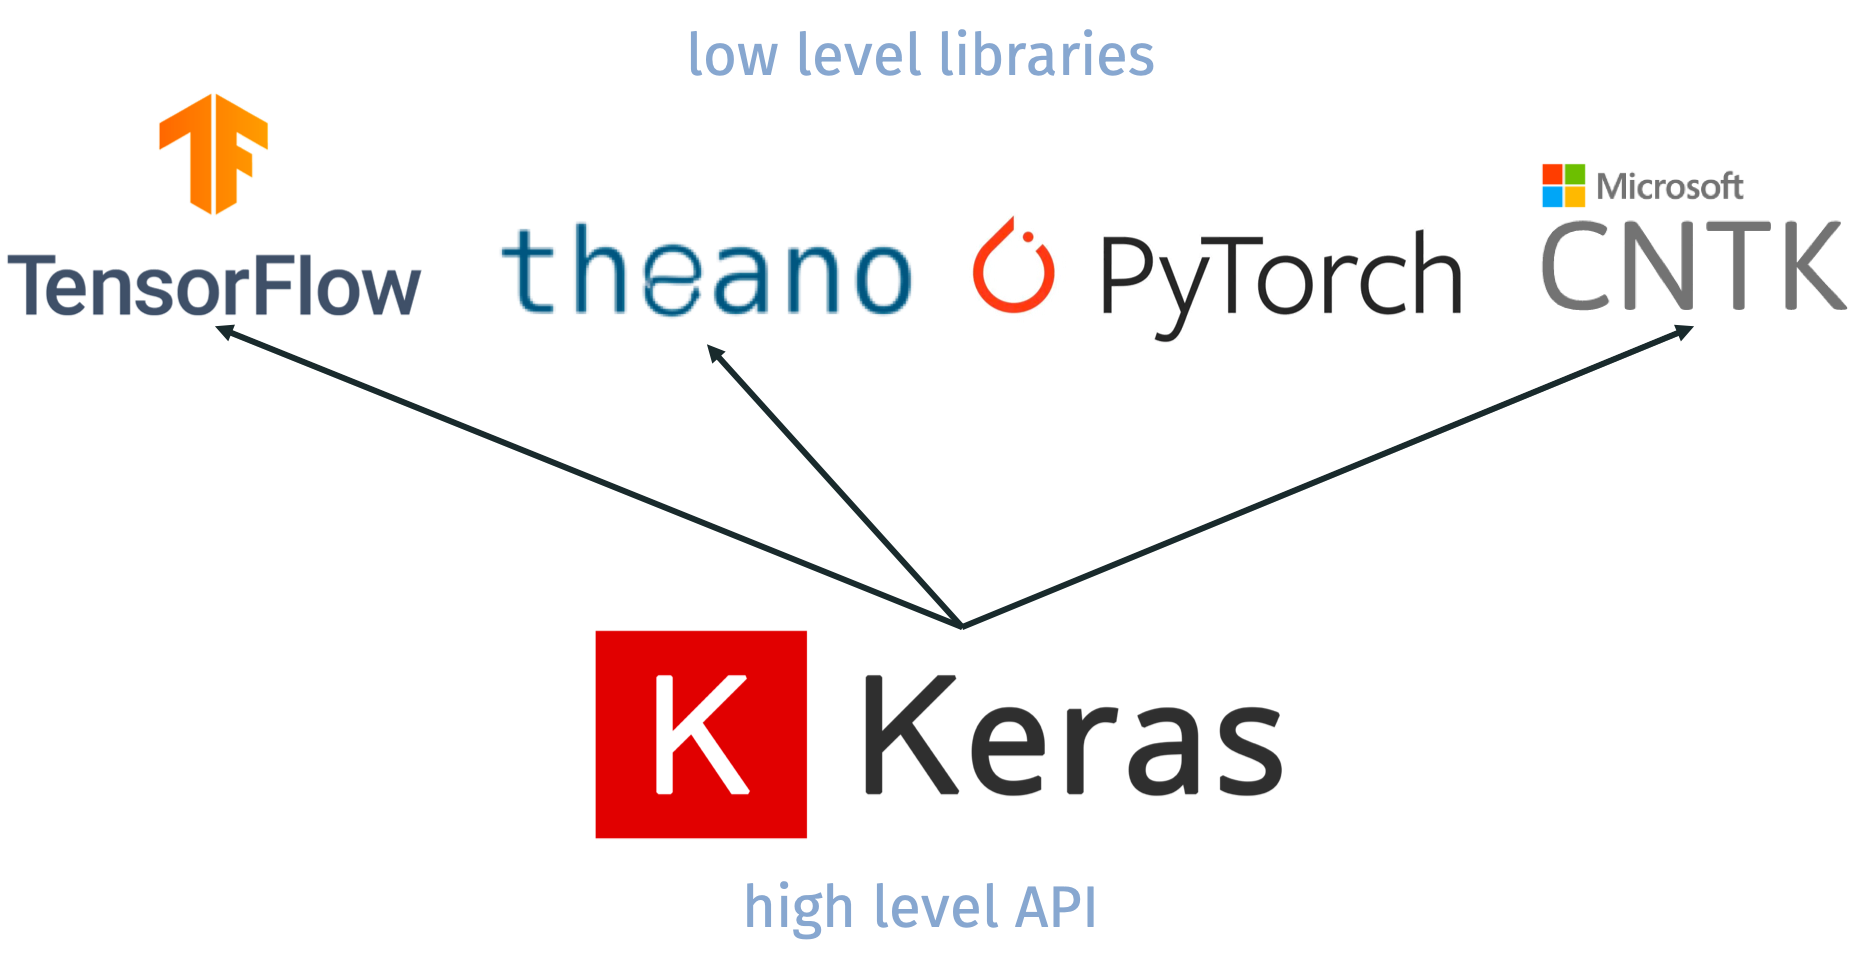
\includegraphics[width=.9\textwidth]{neural_net_zoo.png}
	\end{center}
	\vspace{-1em}

	\textbf{Low-level libraries} have built in optimizers (SGD and improvements) and can automatically perform backpropagation for arbitrary network structures. Also ptimize code for any available GPUs.
	
	\textbf{Keras} has high level functions for defining and training a neural network architecture.
	\end{frame}
	
	\begin{frame}
		\frametitle{neural network software}
		\small
		\textbf{Define model:}
		\begin{center}
			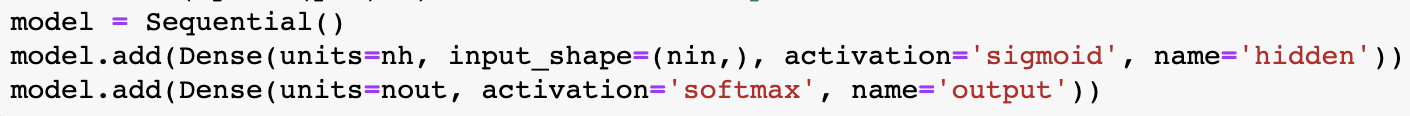
\includegraphics[width=\textwidth]{define_model.png}
		\end{center}
		\vspace{-1em}
		
		\textbf{Compile model:}
		\begin{center}
		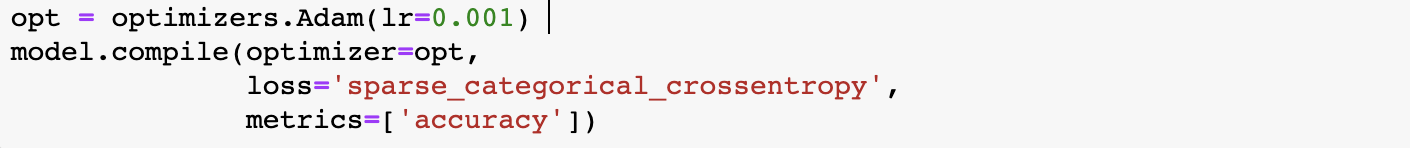
\includegraphics[width=\textwidth]{compile_model.png}
		\end{center}
		\vspace{-1em}
		
		\textbf{Train model:}
		\begin{center}
		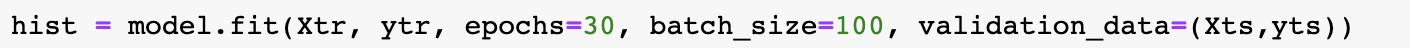
\includegraphics[width=\textwidth]{runmodel.png}
		\end{center}
		\vspace{-1em}
	\end{frame}

	\begin{frame}
	\frametitle{multiclass classification}
	The MNIST demo performs \emph{multiclass classification.} Typically approach to multiclass problems with neural networks is to have one output neuron \emph{per class}:
	\begin{center}
		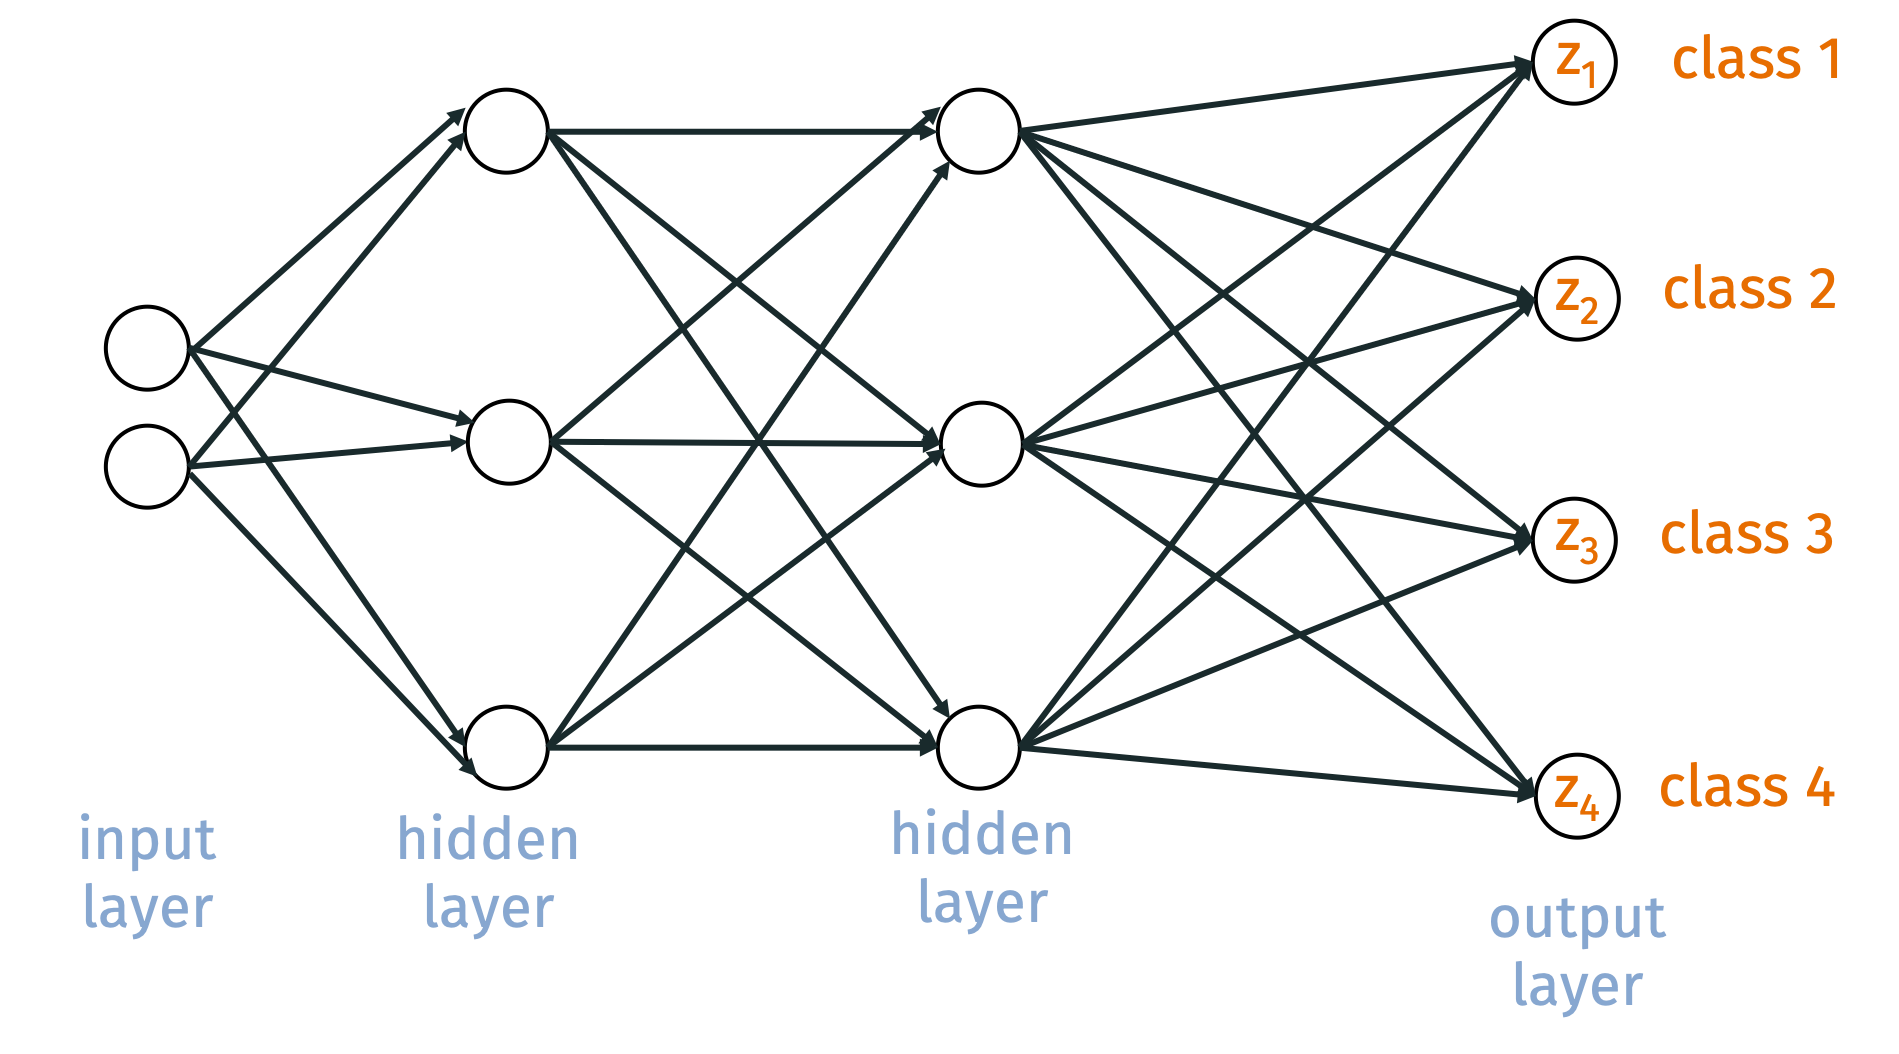
\includegraphics[width=.8\textwidth]{multiclass_network.png}
	\end{center}
	
	\vspace{-1.5em}
	\textbf{Classification rule:} Place in input $\vec{x}$ in class $i$ if $z_i$ is the neuron with maximum value after running $\vec{x}$ through the network.
	\end{frame}

	\begin{frame}
	\frametitle{multiclass classification}
	\begin{center}
		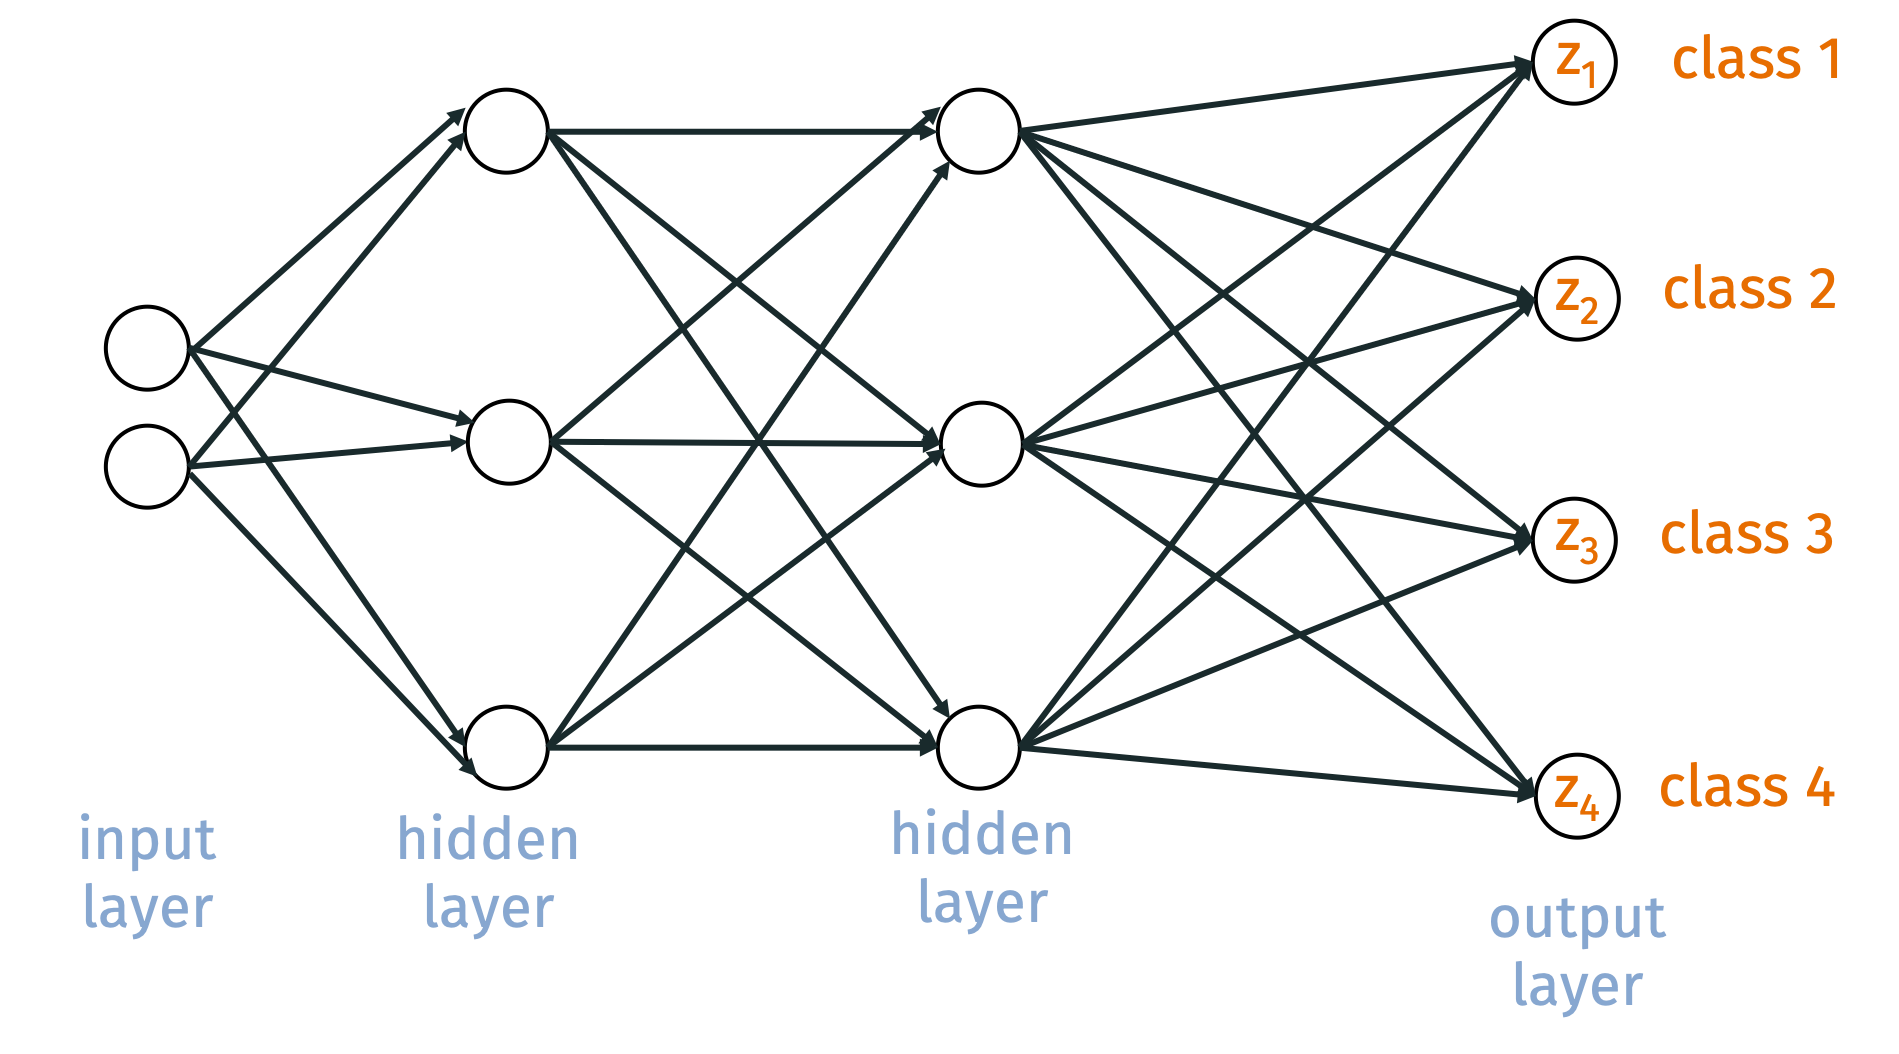
\includegraphics[width=.8\textwidth]{multiclass_network.png}
	\end{center}
Last layer typically uses a ``softmax'' nonlinearity to map all values $\bar{z}_1, \ldots, \bar{z}_q$ to values between $0$ and $1$:
\begin{align*}
z_i = \frac{e^{-\bar{z}_i}}{\sum_{j=1}^q e^{-\bar{z}_j}}.
\end{align*}
	\end{frame}

	\begin{frame}
	\frametitle{multiclass classification}
	Trained using \emph{multiclass cross-entropy loss}. Let $z_1(\vec{x},\theta), \ldots, z_q(\vec{x},\theta)$ be the outputs obtain when running the network on input $\vec{x}$ with parameters (weights and baises) $\vec{\theta}$. 
	\begin{align*}
	L(y, \vec{x}, \vec{\theta}) = - \sum_{i=1}^q \mathbbm{1}[y = i] \log(z_i(\vec{x},\theta)).
	\end{align*}
	
	Overall loss for training data $(\vec{x}_1, y_1), \ldots, (\vec{x}_n, y_n)$ is:
	\begin{align*}
	\mathcal{L}(\vec{\theta}) = \sum_{i=1}^n L(y_i, \vec{x}_i, \vec{\theta})
	\end{align*}
	\begin{center}
		\alert{\textbf{Used in our demo and very standard for neural network classification.}}
	\end{center}
	\end{frame}

	\begin{frame}
	\frametitle{feature extraction}
	\begin{center}
	\textbf{Why do neural networks work so well?}
	\end{center}
	Treat feature transformation/extraction as \emph{part of the learning process} instead of making this the users job.
	
	But sometimes they still need a nudge in the right direction...
	\end{frame}

	\begin{frame}
		\frametitle{basic feature extraction}		
		\begin{center}
			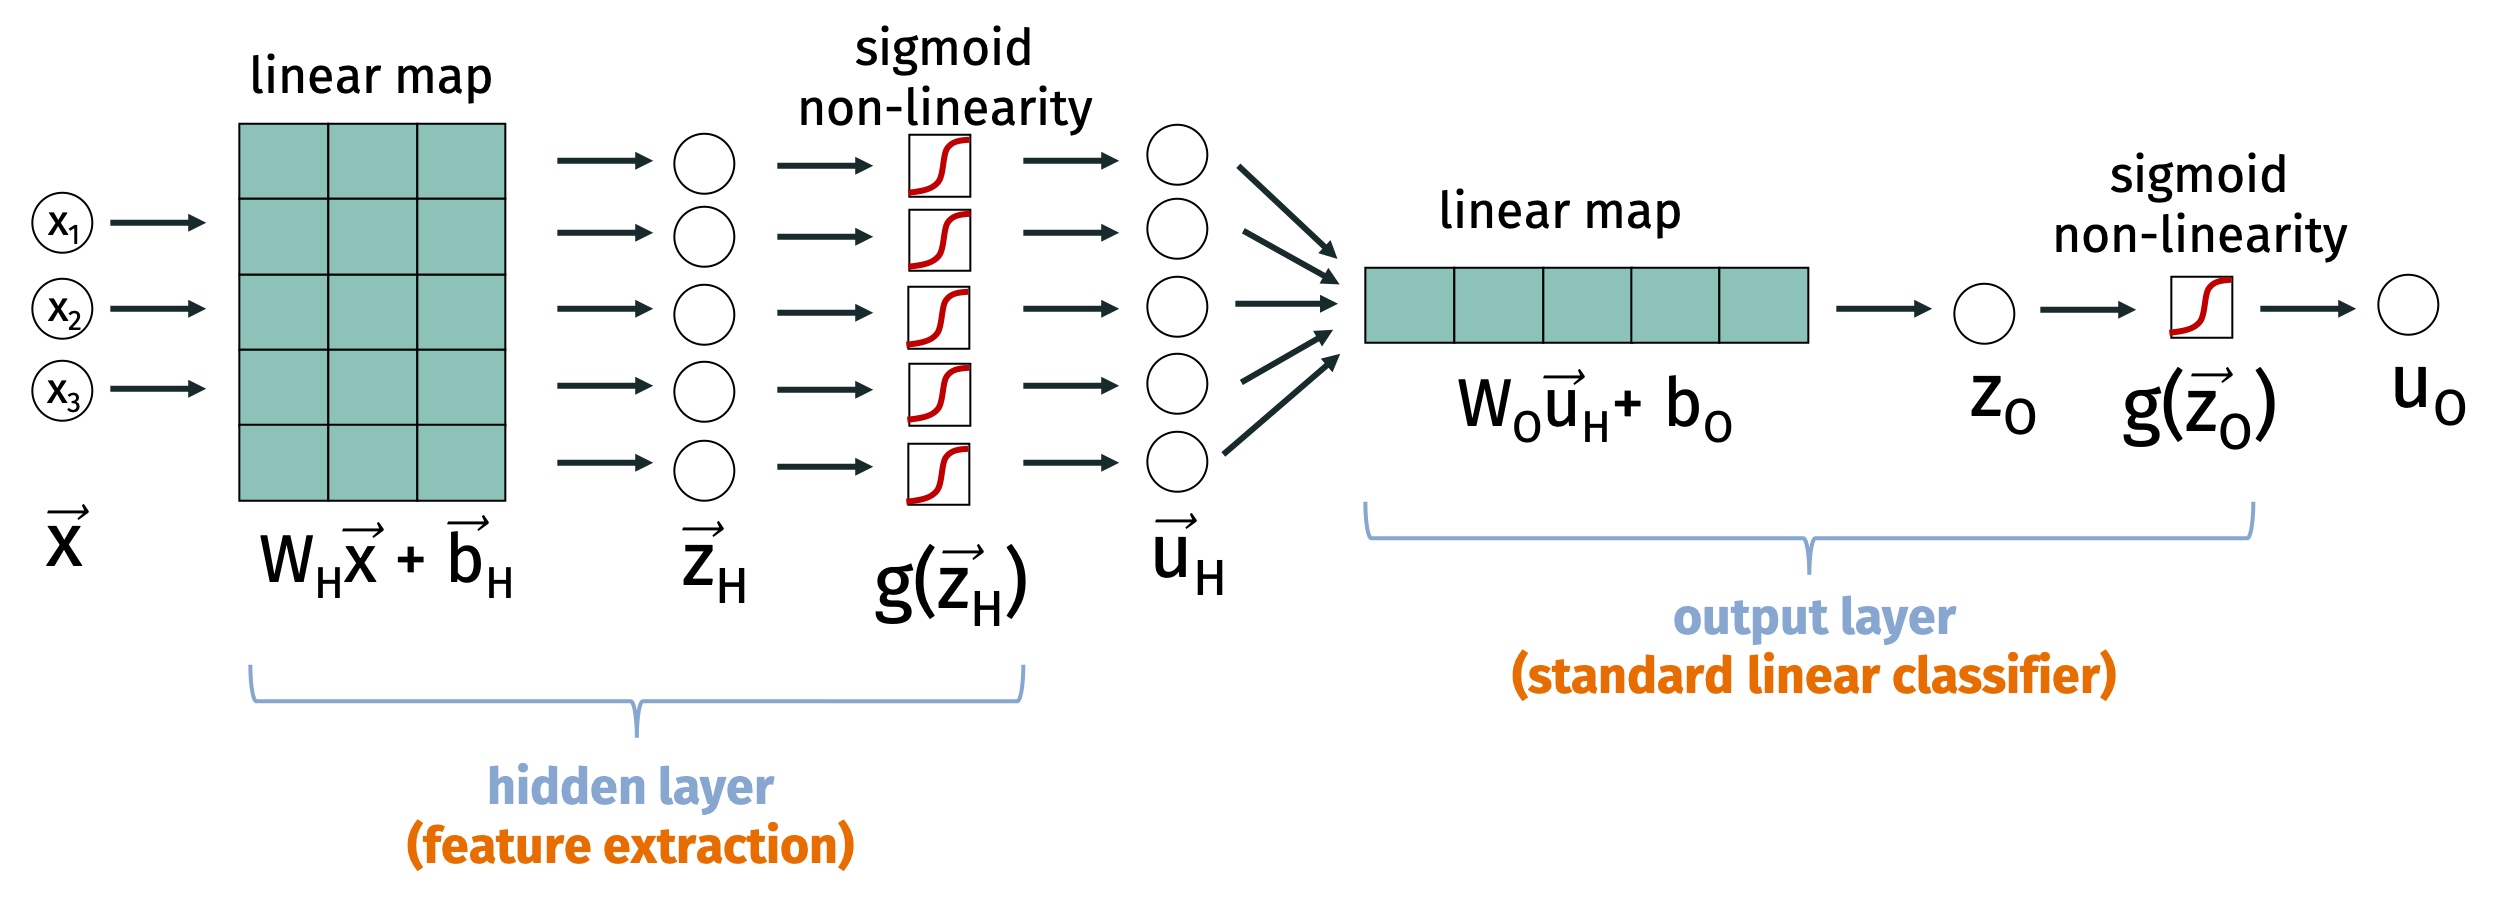
\includegraphics[width=\textwidth]{neural_net_arch.png}
		\end{center}	
	\end{frame}

	\begin{frame}
	\frametitle{basic feature extraction}		
	\begin{center}
		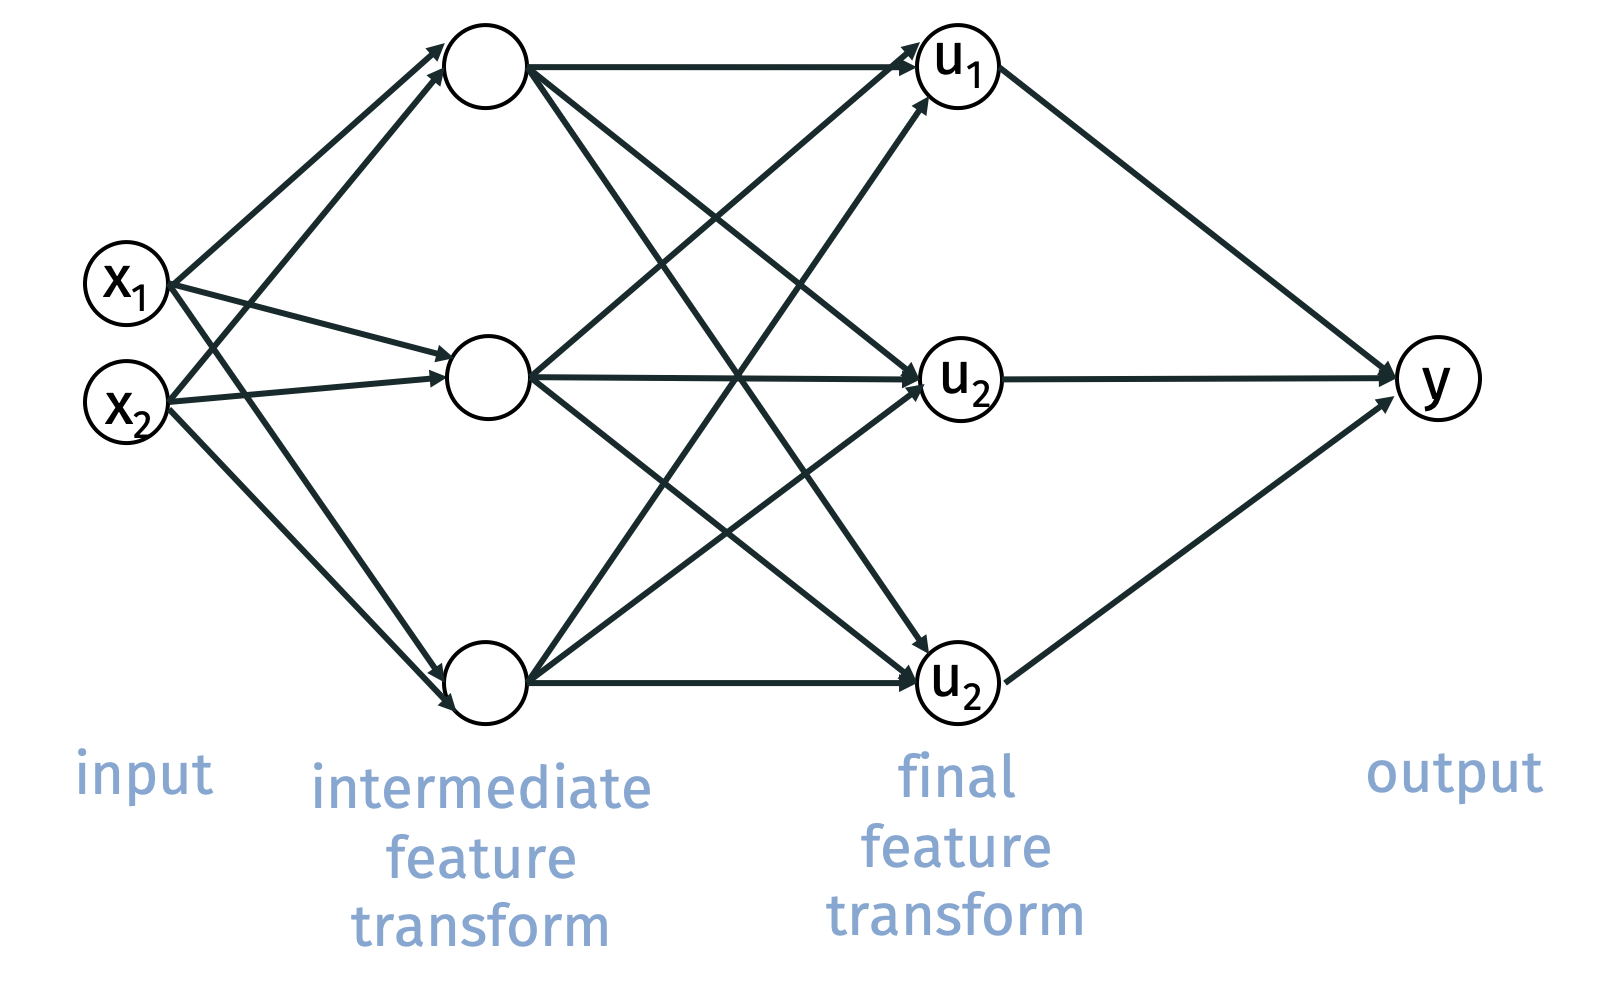
\includegraphics[width=.7\textwidth]{3layer.png}
	\end{center}	
	Final output or class label $y$ is a \emph{linear function} of the final layer variables $u_1, \ldots, u_k$. You could just as well have taken these variables and used them to predict $y$ via linear regression, logistic regression, SVM, any other linear method.
	\end{frame}

	\begin{frame}
	\frametitle{basic feature extraction}
	\textbf{Sigmoid activation:} Each hidden variable $z_i$ equal to $\frac{1}{1 + e^{-\bar{z}_i}}$ where $z_i = \vec{w}^T\vec{x} + b$ for input $\vec{x}$. 
		\begin{center}
			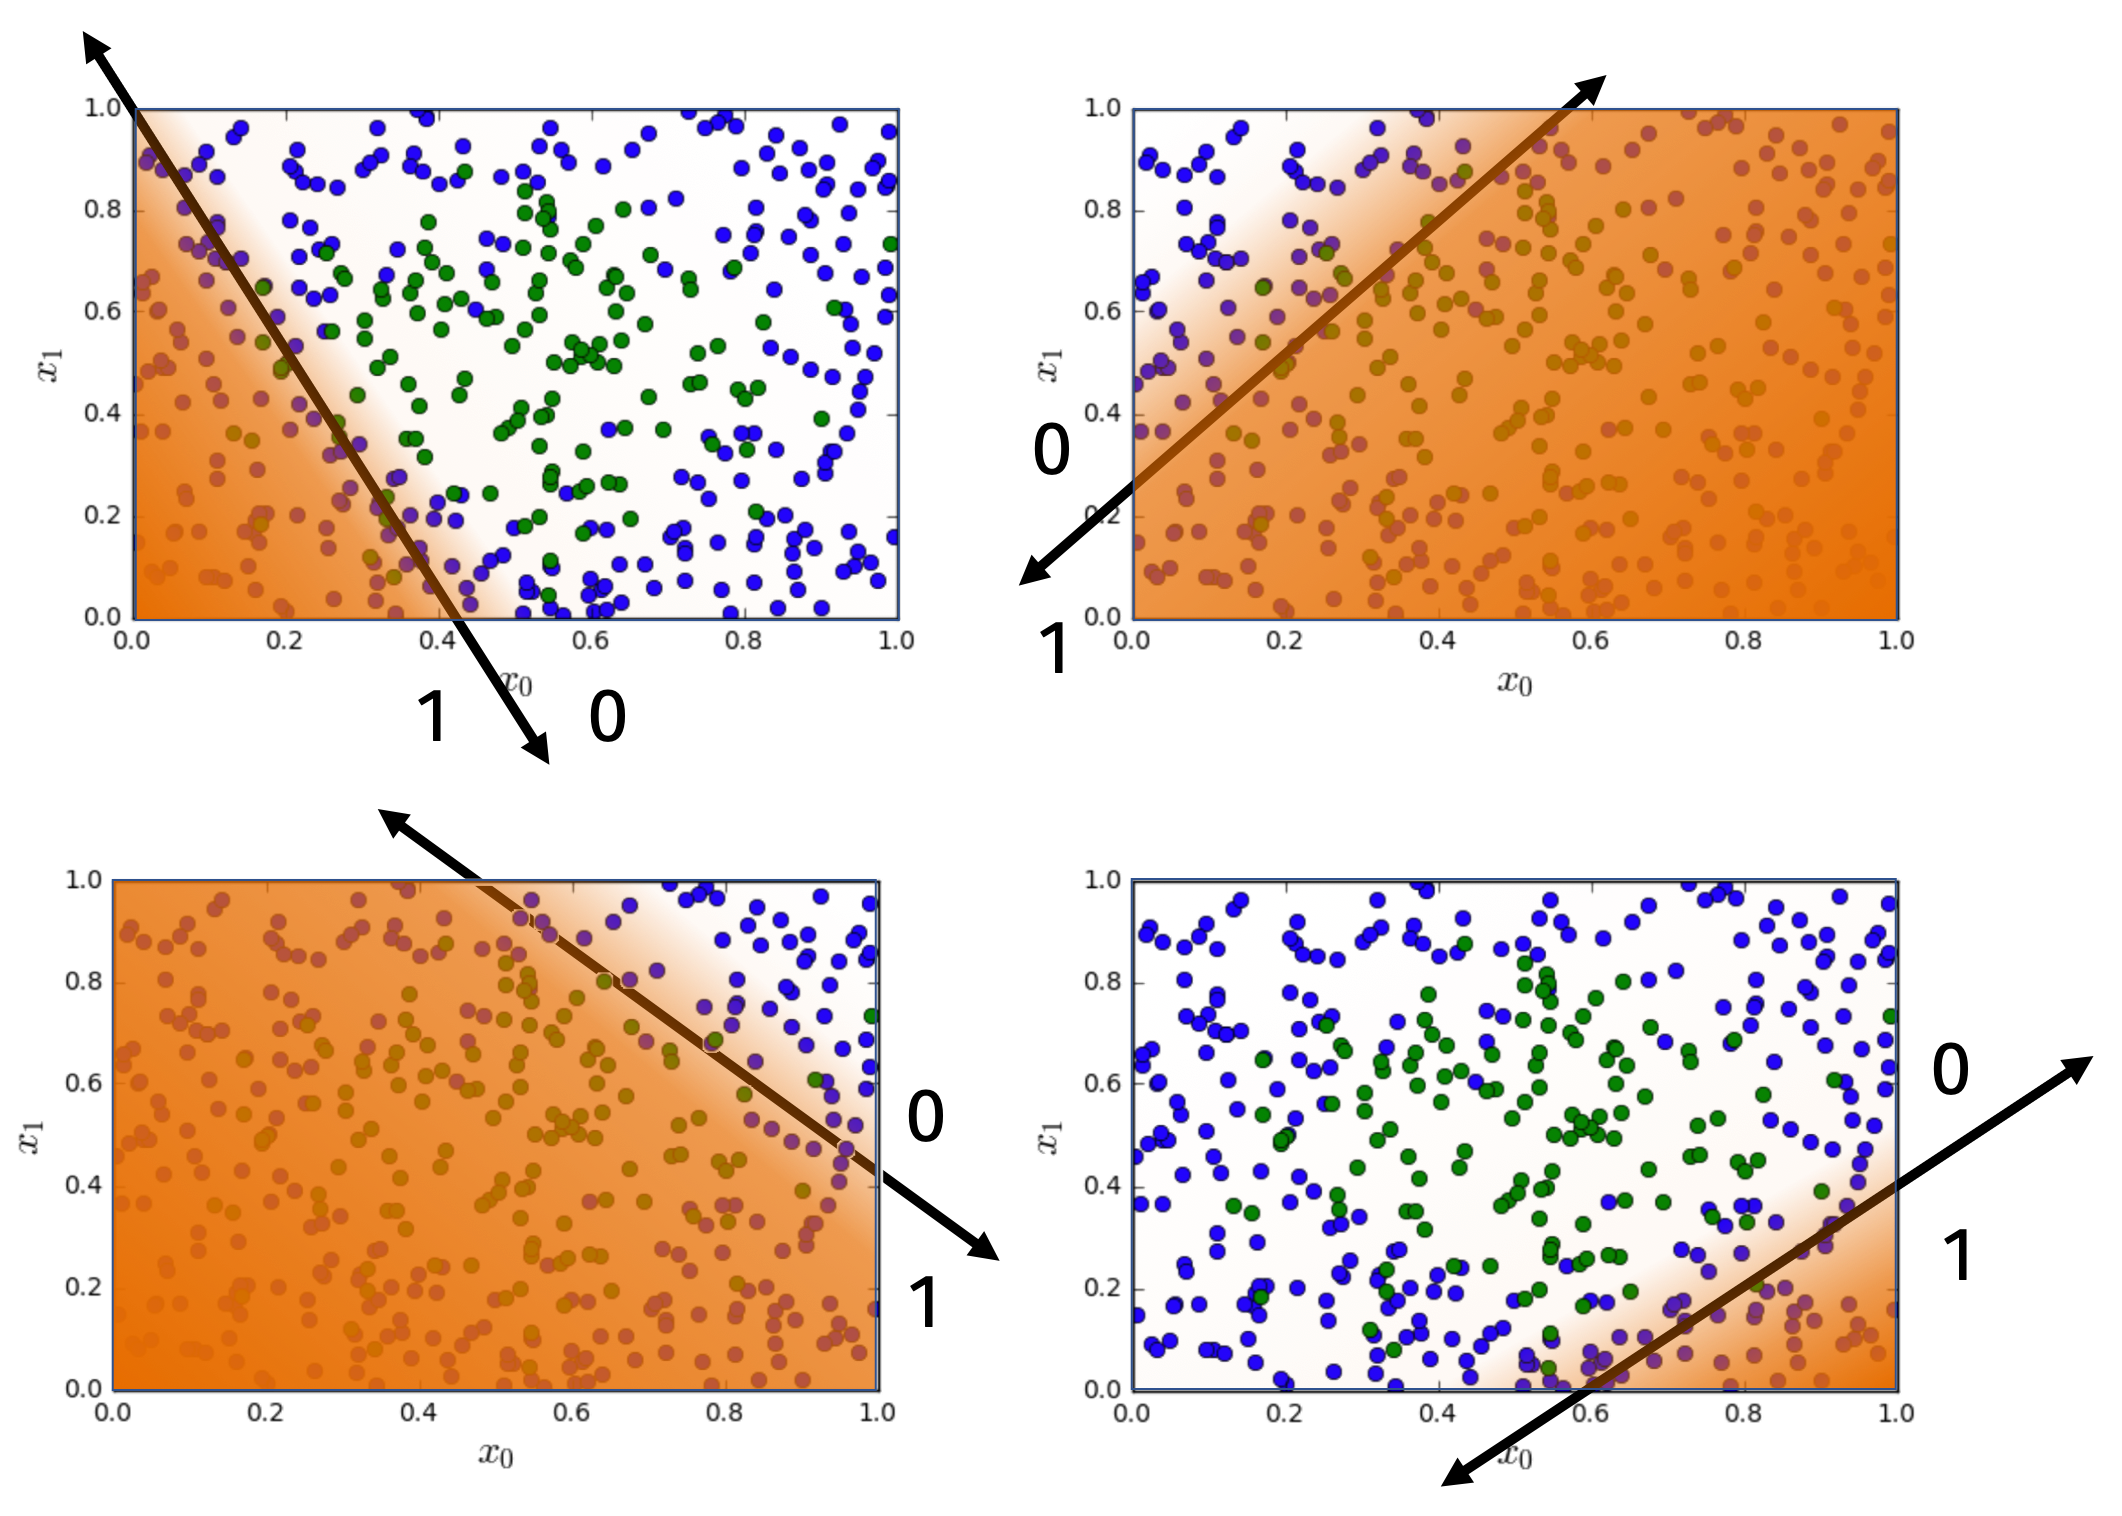
\includegraphics[width=.6\textwidth]{soft_features.png}
		\end{center}	
	Other non-linearities yield similarly simple feature extractions. 
	\end{frame}

	\begin{frame}
	\frametitle{basic feature extraction}
	If you combine more hidden variables, you can start building more complicated classifiers.
	\begin{center}
		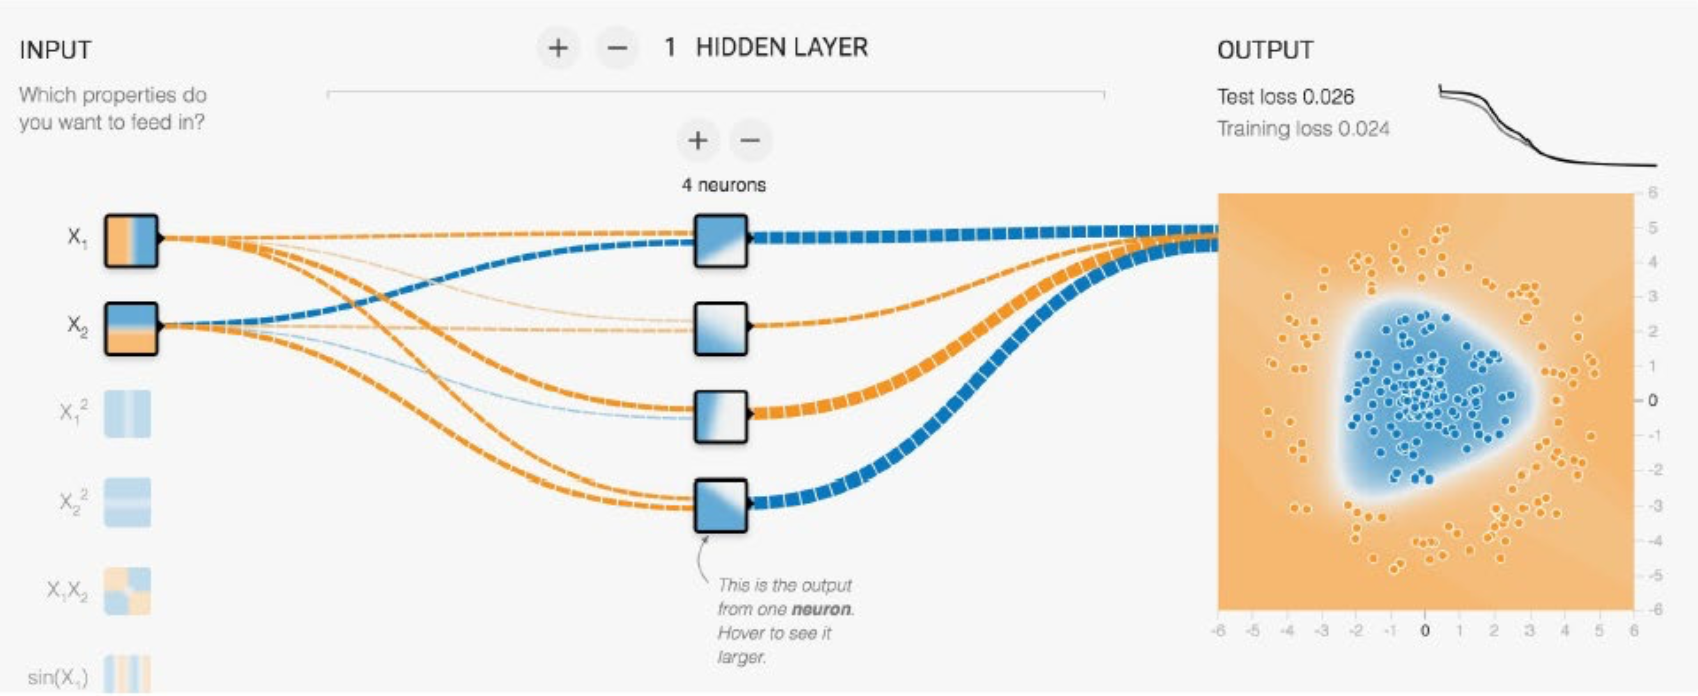
\includegraphics[width=.55\textwidth]{power1.png}
	\end{center}
How about for even more complex datasets?
\vspace{-.5em}
	\begin{center}
	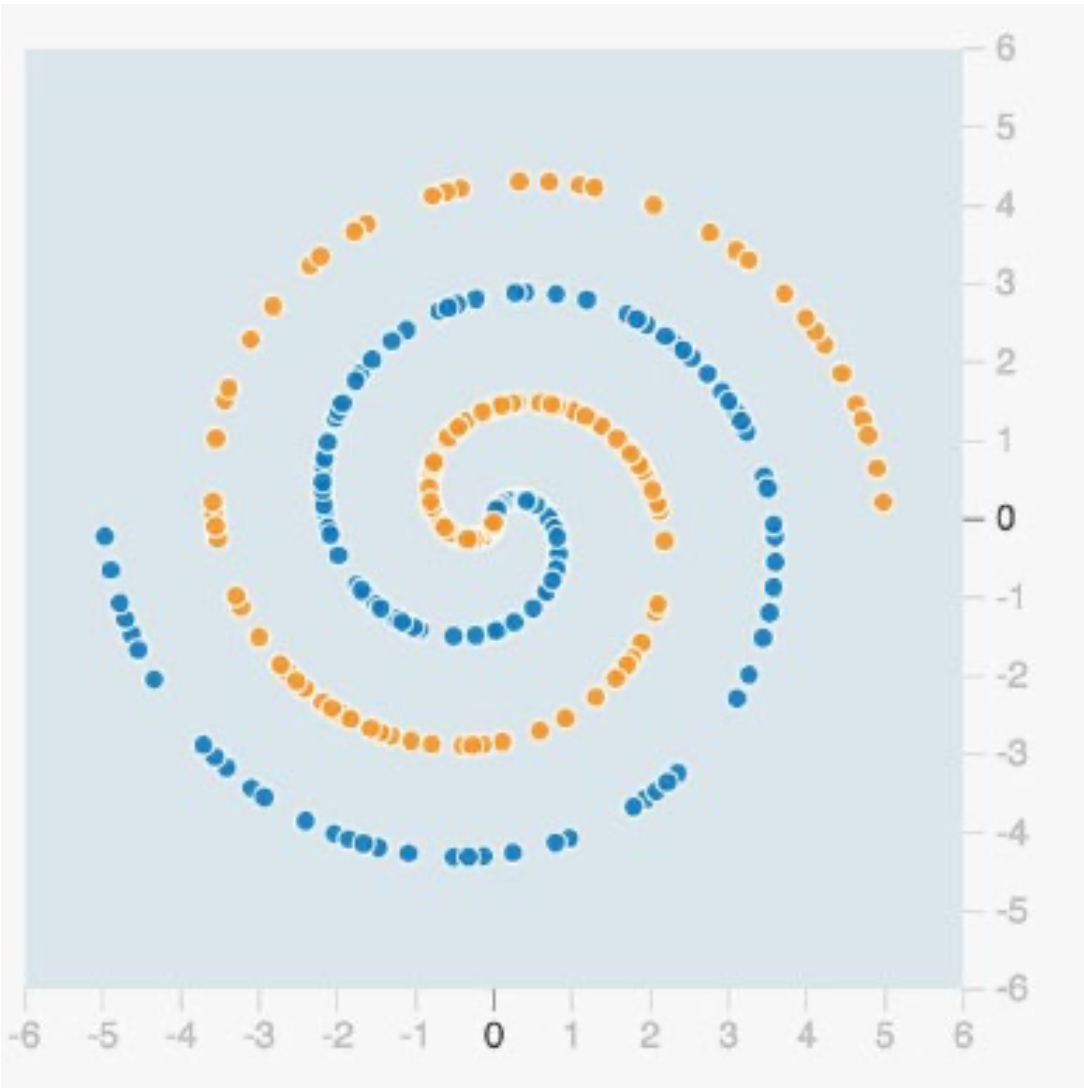
\includegraphics[width=.3\textwidth]{spiral.png}
	\end{center}
	\end{frame}

	\begin{frame}
	\frametitle{basic feature extraction}
	With more layers, complexity starts ramping up...
	\begin{center}
		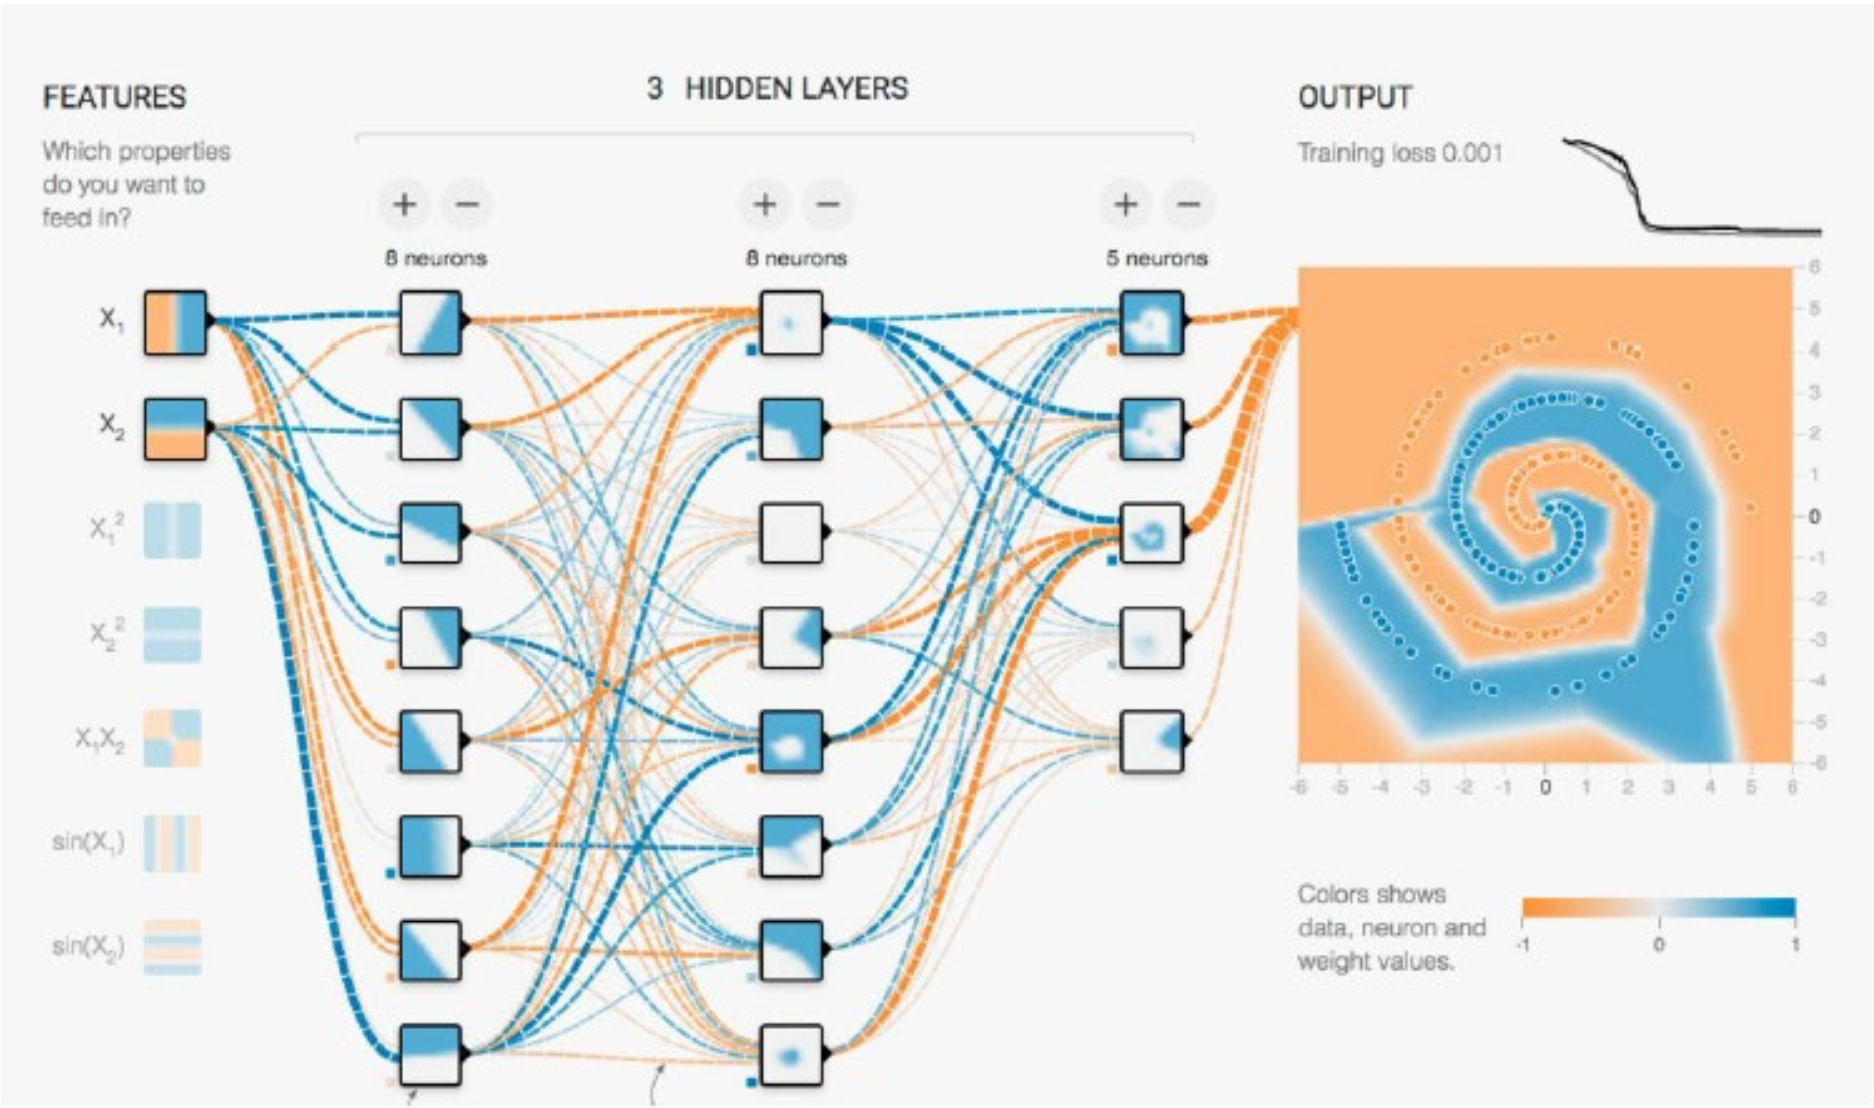
\includegraphics[width=.8\textwidth]{power2.png}
	\end{center}
But there's a limit...
	\end{frame}

	\begin{frame}
	\frametitle{basic feature extraction}
	Modern machine learning algorithms can differentiate between images of African and Asian elephants...
	\begin{center}
		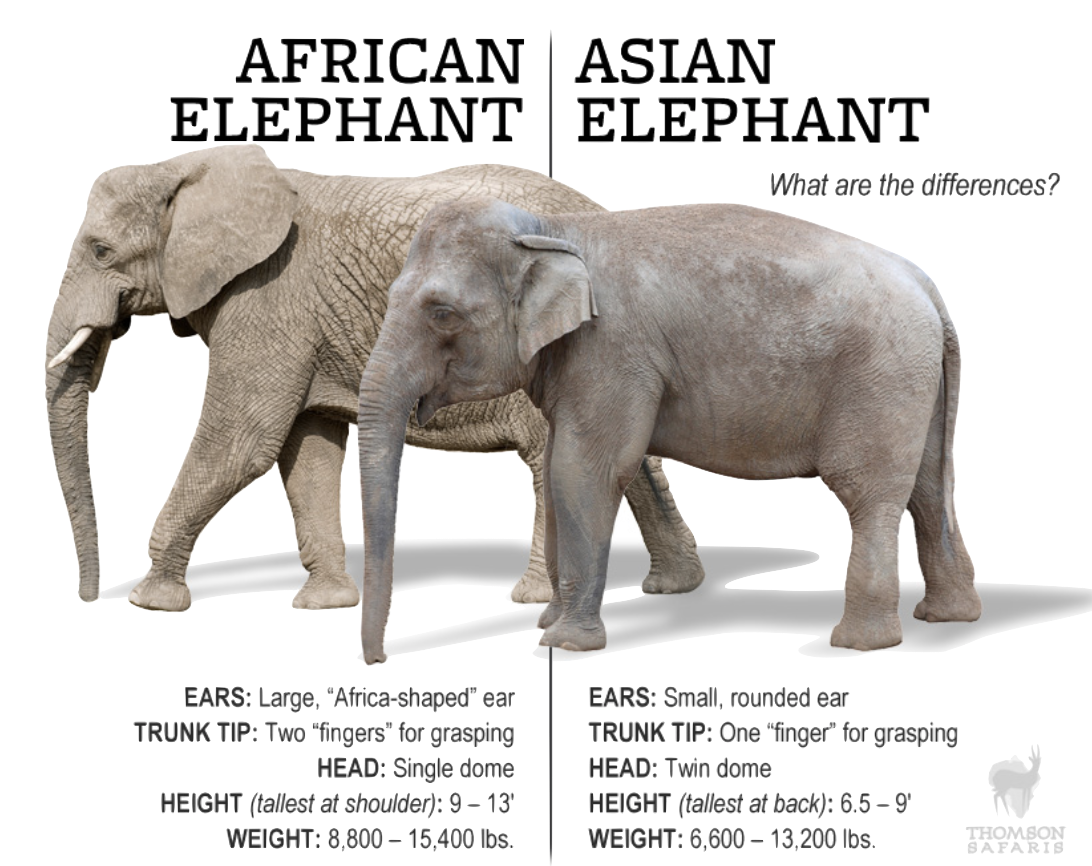
\includegraphics[width=.5\textwidth]{elephants.png}
	\end{center}
The features needed for a task like this are \emph{far more complex} then we could expect a network to learn completely on its own using simple combinations of linear layers + non-linearities. 
	\end{frame}

	\begin{frame}
	\frametitle{convolutional feature extraction}
	\textbf{Today's topic:} Understand why \emph{convolution} is a powerful way of extracting features from:
	\begin{itemize}
		\item Image data.
		\item Audio data.
		\item Time series data.
	\end{itemize}
	Ultimately, can build \emph{convolutional networks} that already have convolutional feature extraction \emph{pre-coded in}. Just need to learn weights. 
	\end{frame}

	\begin{frame}
	\frametitle{motivating example}
	What features would tell use this image contains a stop sign?
	\begin{center}
		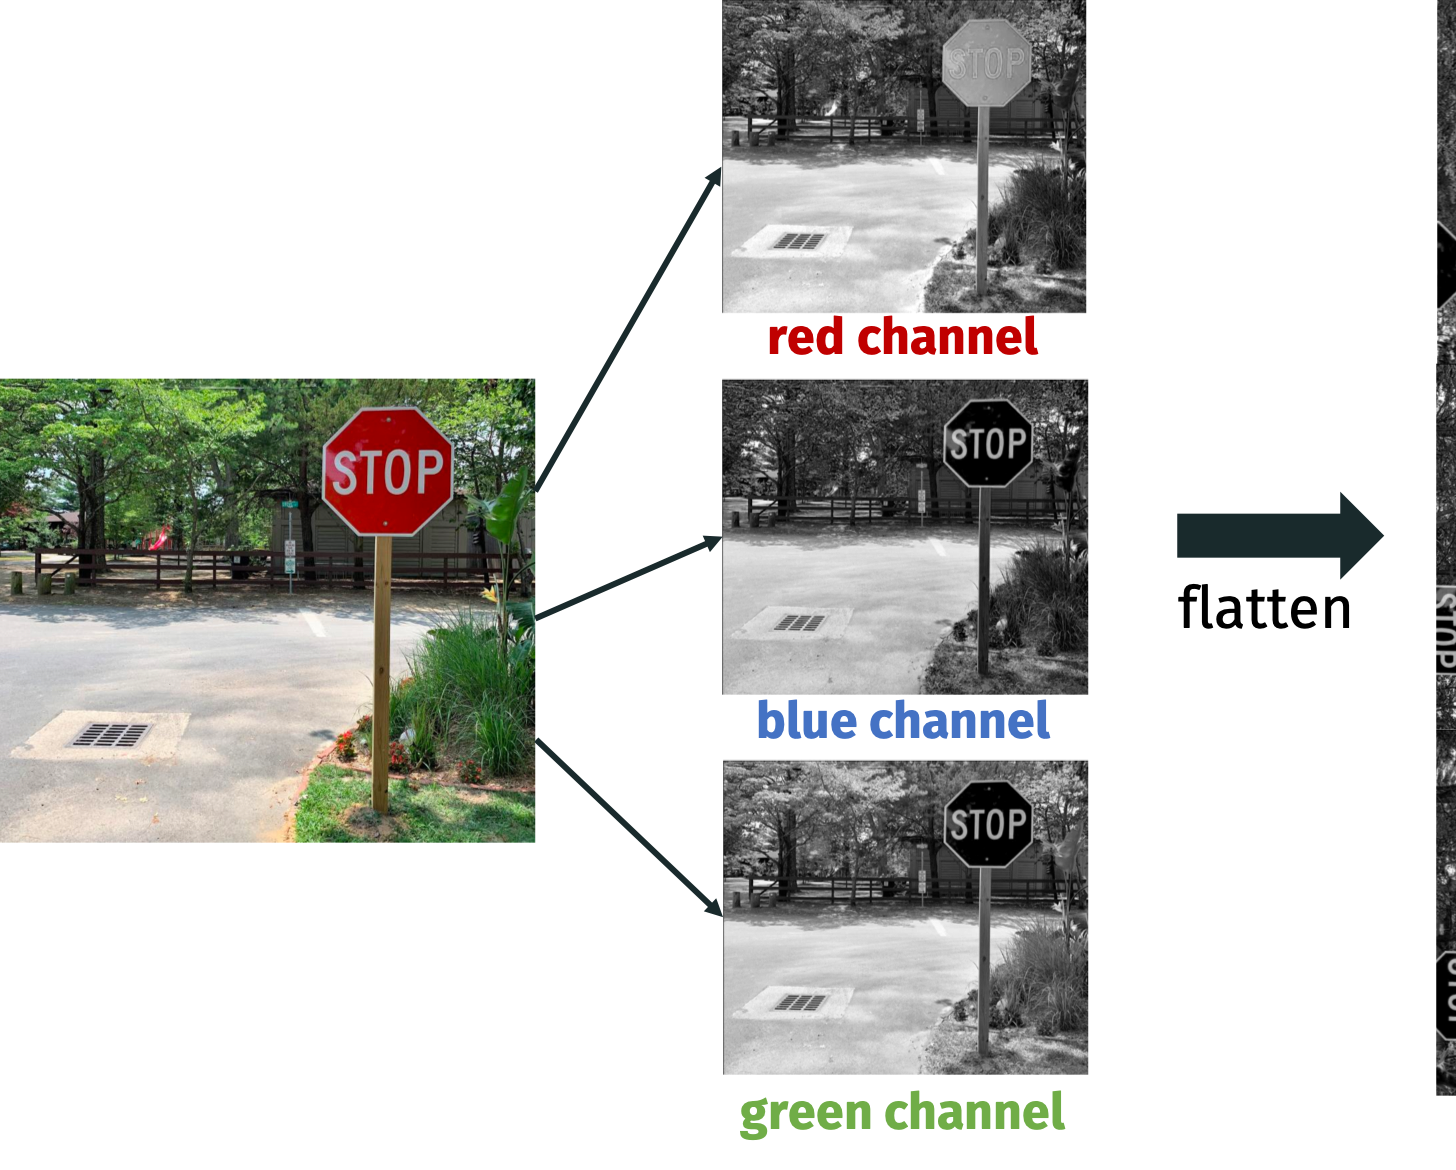
\includegraphics[width=.6\textwidth]{stopsign_flat.png}
	\end{center}
Typically way of vectorizing an image chops up and splits up any pixels in the stop sign. We need very complex features to piece these back together again...
	\end{frame}

	\begin{frame}
	\frametitle{convolution}
	\small
	Objects or features of an image often involve pixels that are \emph{spatially correlated.} Convolution explicitly encodes this.
	
	\begin{definition}[Discrete 1D convolution\footnote{This is slightly different from the definition of convolution you might have seen in a Digital Signal Processing class because $\vec{w}$ does not get ``flipped". In signal processing our operation would be called \emph{correlation}.}]
	Given $\vec{x} \in \R^d$ and $\vec{w} \in \R^k$ the discrete convolution $\vec{x}\circledast\vec{w}$ is a $d - k + 1$ vector with:
	\vspace{-1em}
	\begin{align*}
	[\vec{x}\circledast\vec{w}]_i = \sum_{j=1}^k \vec{x}_{(j+i-1)}\vec{w}_{j}
	\end{align*}
		\vspace{-1em}
	\end{definition}
	Think of $\vec{x} \in \R^d$ as long \textbf{data vector} (e.g. d = 512) and $\vec{w} \in \R^k$ as short \textbf{filter vector} (e.g. k = 8). $\vec{u} = [\vec{x}\circledast\vec{w}]$ is a feature transformation.
	\end{frame}

	\begin{frame}
	\frametitle{1d convolution}
	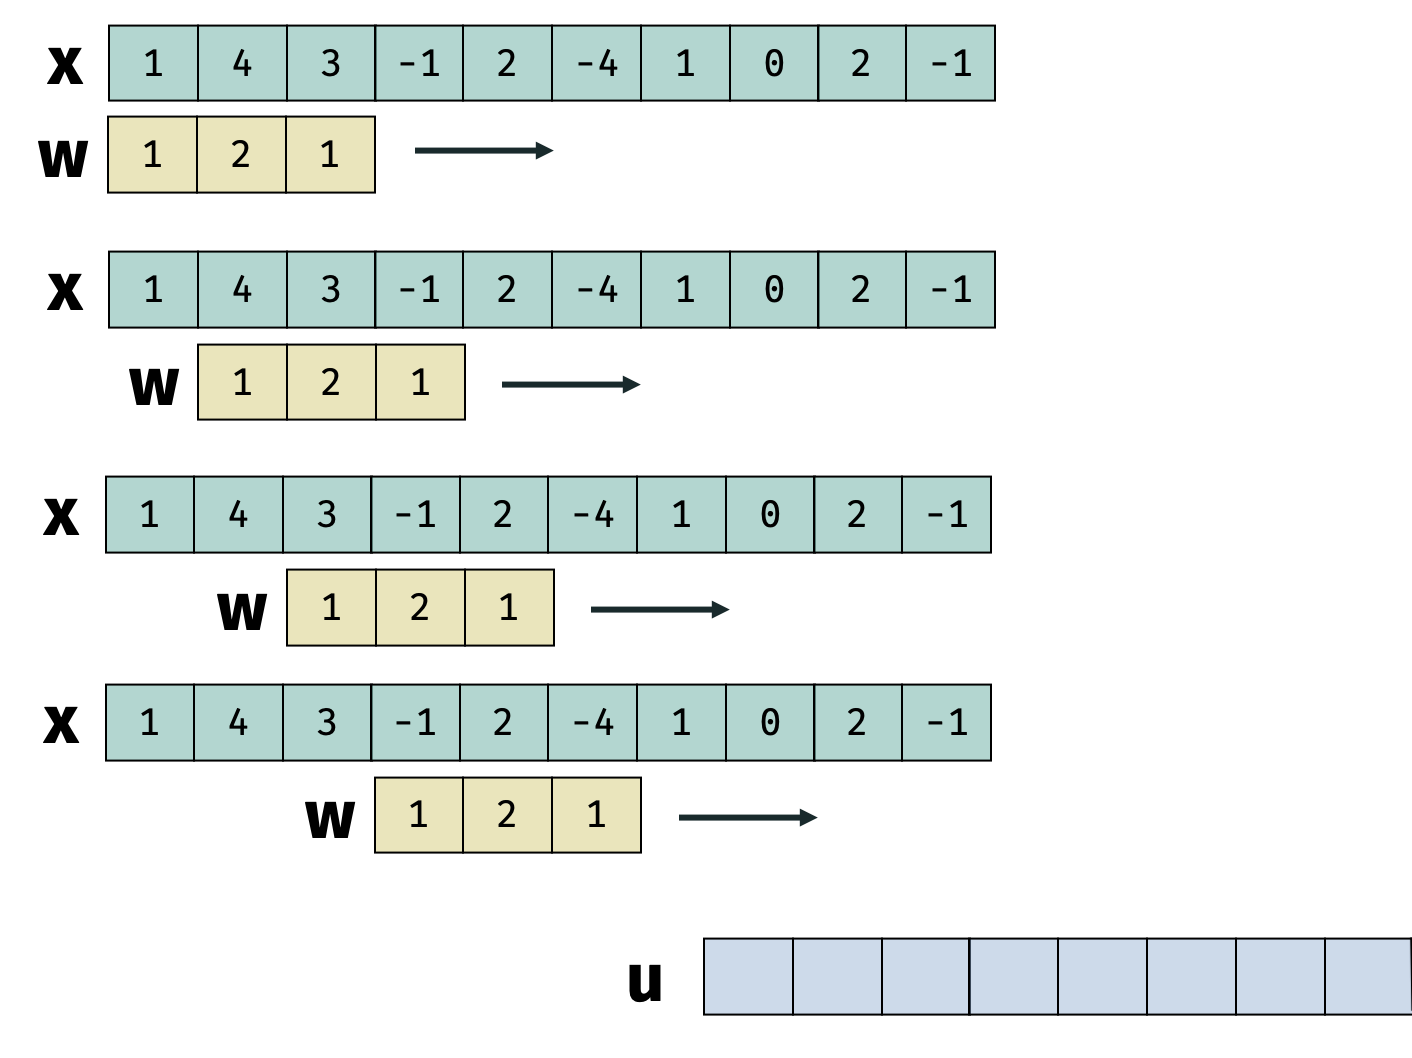
\includegraphics[width=.9\textwidth]{1d_conv_examp.png}
	\end{frame}

	\begin{frame}
	\frametitle{match the convolution}
	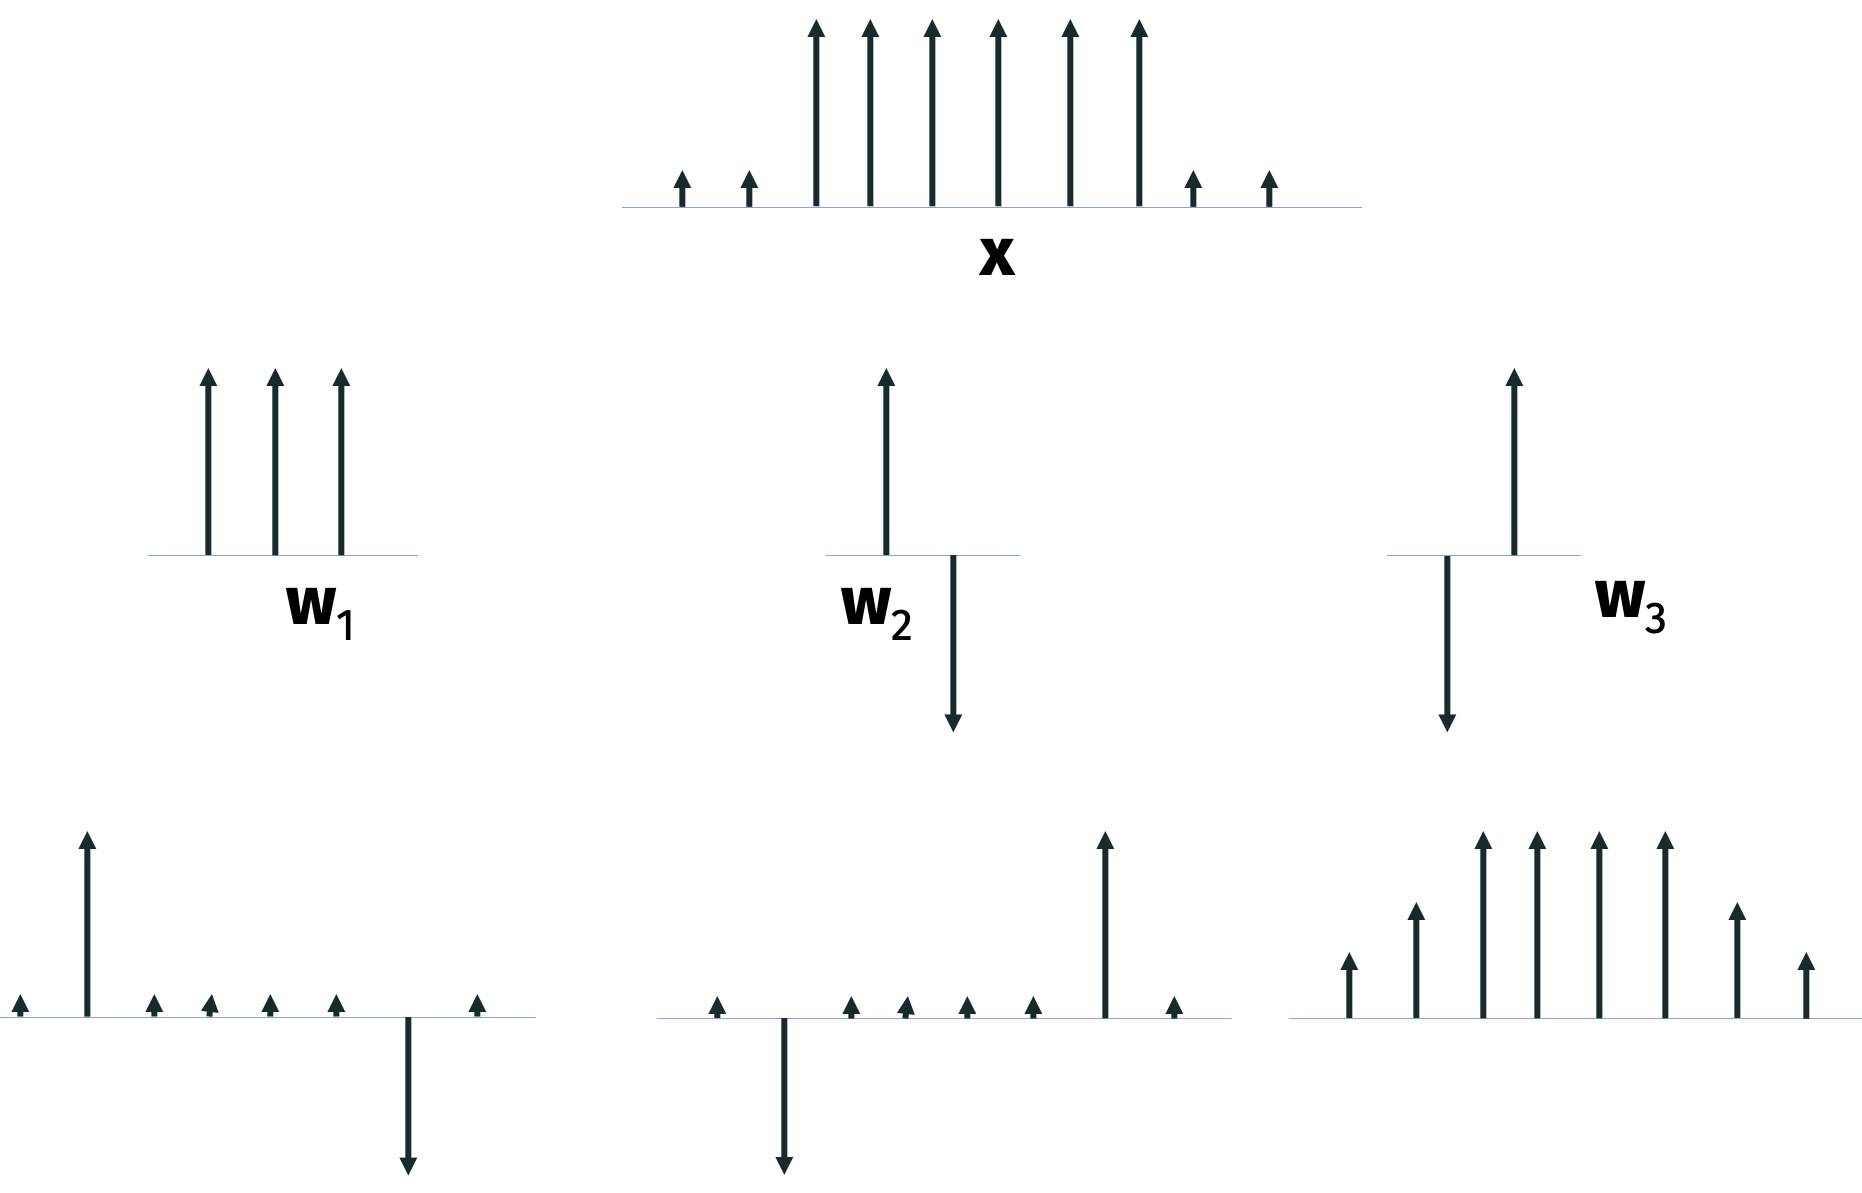
\includegraphics[width=\textwidth]{match.png}
	\end{frame}

	\begin{frame}
		\frametitle{2d convolution}
			\small
			\begin{definition}[Discrete 2D convolution]
				Given matrices $\bv{x} \in \R^{d_1\times d_2}$ and $\bv{w} \in \R^{k_1\times k_2}$ the discrete convolution $\bv{x}\circledast \bv{w}$ is a $(d_1 - k_1 + 1)\times (d_2 - k_2 + 1)$ matrix with:
				\vspace{-1em}
				\begin{align*}
				[\bv{x}\circledast \bv{w}]_{i,j} = \sum_{\ell=1}^{k_1}\sum_{h=1}^{k_2} \bv{x}_{(i + \ell -1),(j + h -1)}\cdot \bv{w}_{\ell,h}
				\end{align*}
				\vspace{-1em}
			\end{definition}
		
		Again technically this is ``correlation'' not ``convolution''. Should be performed in Python using \texttt{scipy.signal.correlate2d} instead of \texttt{scipy.signal.convolve2d}.
		
		$\bv{w}$ is called the \emph{filter} or \emph{convolution kernel} and again is typically much smaller than $\bv{x}$. 
	\end{frame}

	\begin{frame}
	\frametitle{2d convolution}s
	\small\centering
	$\bv{w} = \begin{bmatrix}0&1&2\\2&2&0\\0&1&2\end{bmatrix}$ 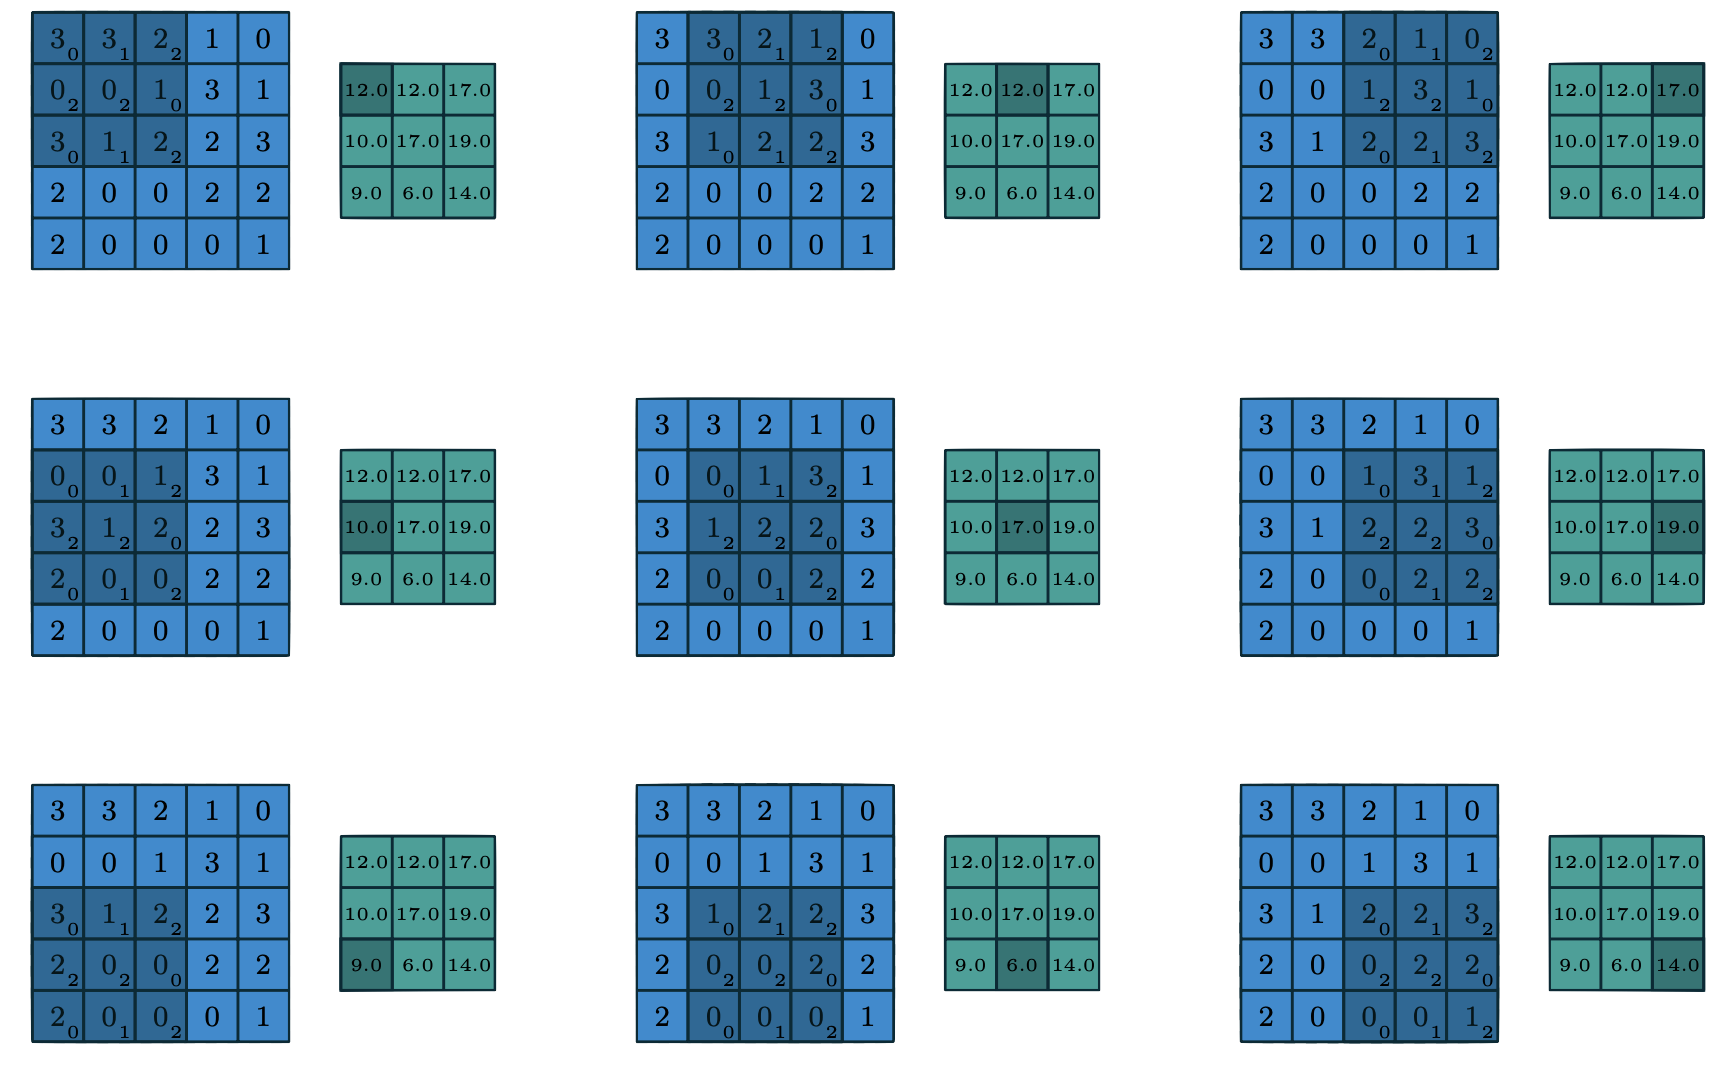
\includegraphics[width=.9\textwidth]{standard2d.png}
	\end{frame}

	\begin{frame}
	\frametitle{zero padding}
	Sometimes ``zero-padding'' is introduced so $\bv{x}\circledast \bv{w}$ is $d_1\times d_2$ if $\bv{x}$ is $d_1\times d_2$.
	
	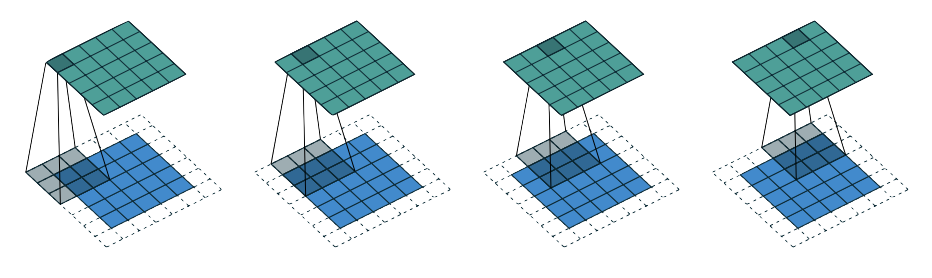
\includegraphics[width=.8\textwidth]{better_zero_pad.png} 
	
	Need to pad on left and right by $(k_1-1)/2$ and on top and bottom by $(k_2 - 1)/2$. 
	\end{frame}

	\begin{frame}
	\frametitle{applications of convolution}
		\begin{center}
			Examples code will be available in \texttt{demo1\_convolutions.ipynb}.
		\end{center}
		\textbf{Application 1:} Blurring/smooth.
		
		In one dimension:
		\begin{itemize}
			\item Uniform (moving average) filter: $\vec{w}_i = \frac{1}{k}$ for $i = 1,\ldots, k$.
			\item Gaussian filter: $\vec{w}_i \sim \exp^{(i-k/2)^2/\sigma^2}$ for $i = 1,\ldots, k$.
		\end{itemize}
	\end{frame}

	\begin{frame}
	\frametitle{smoothing filters}
	\begin{center}
		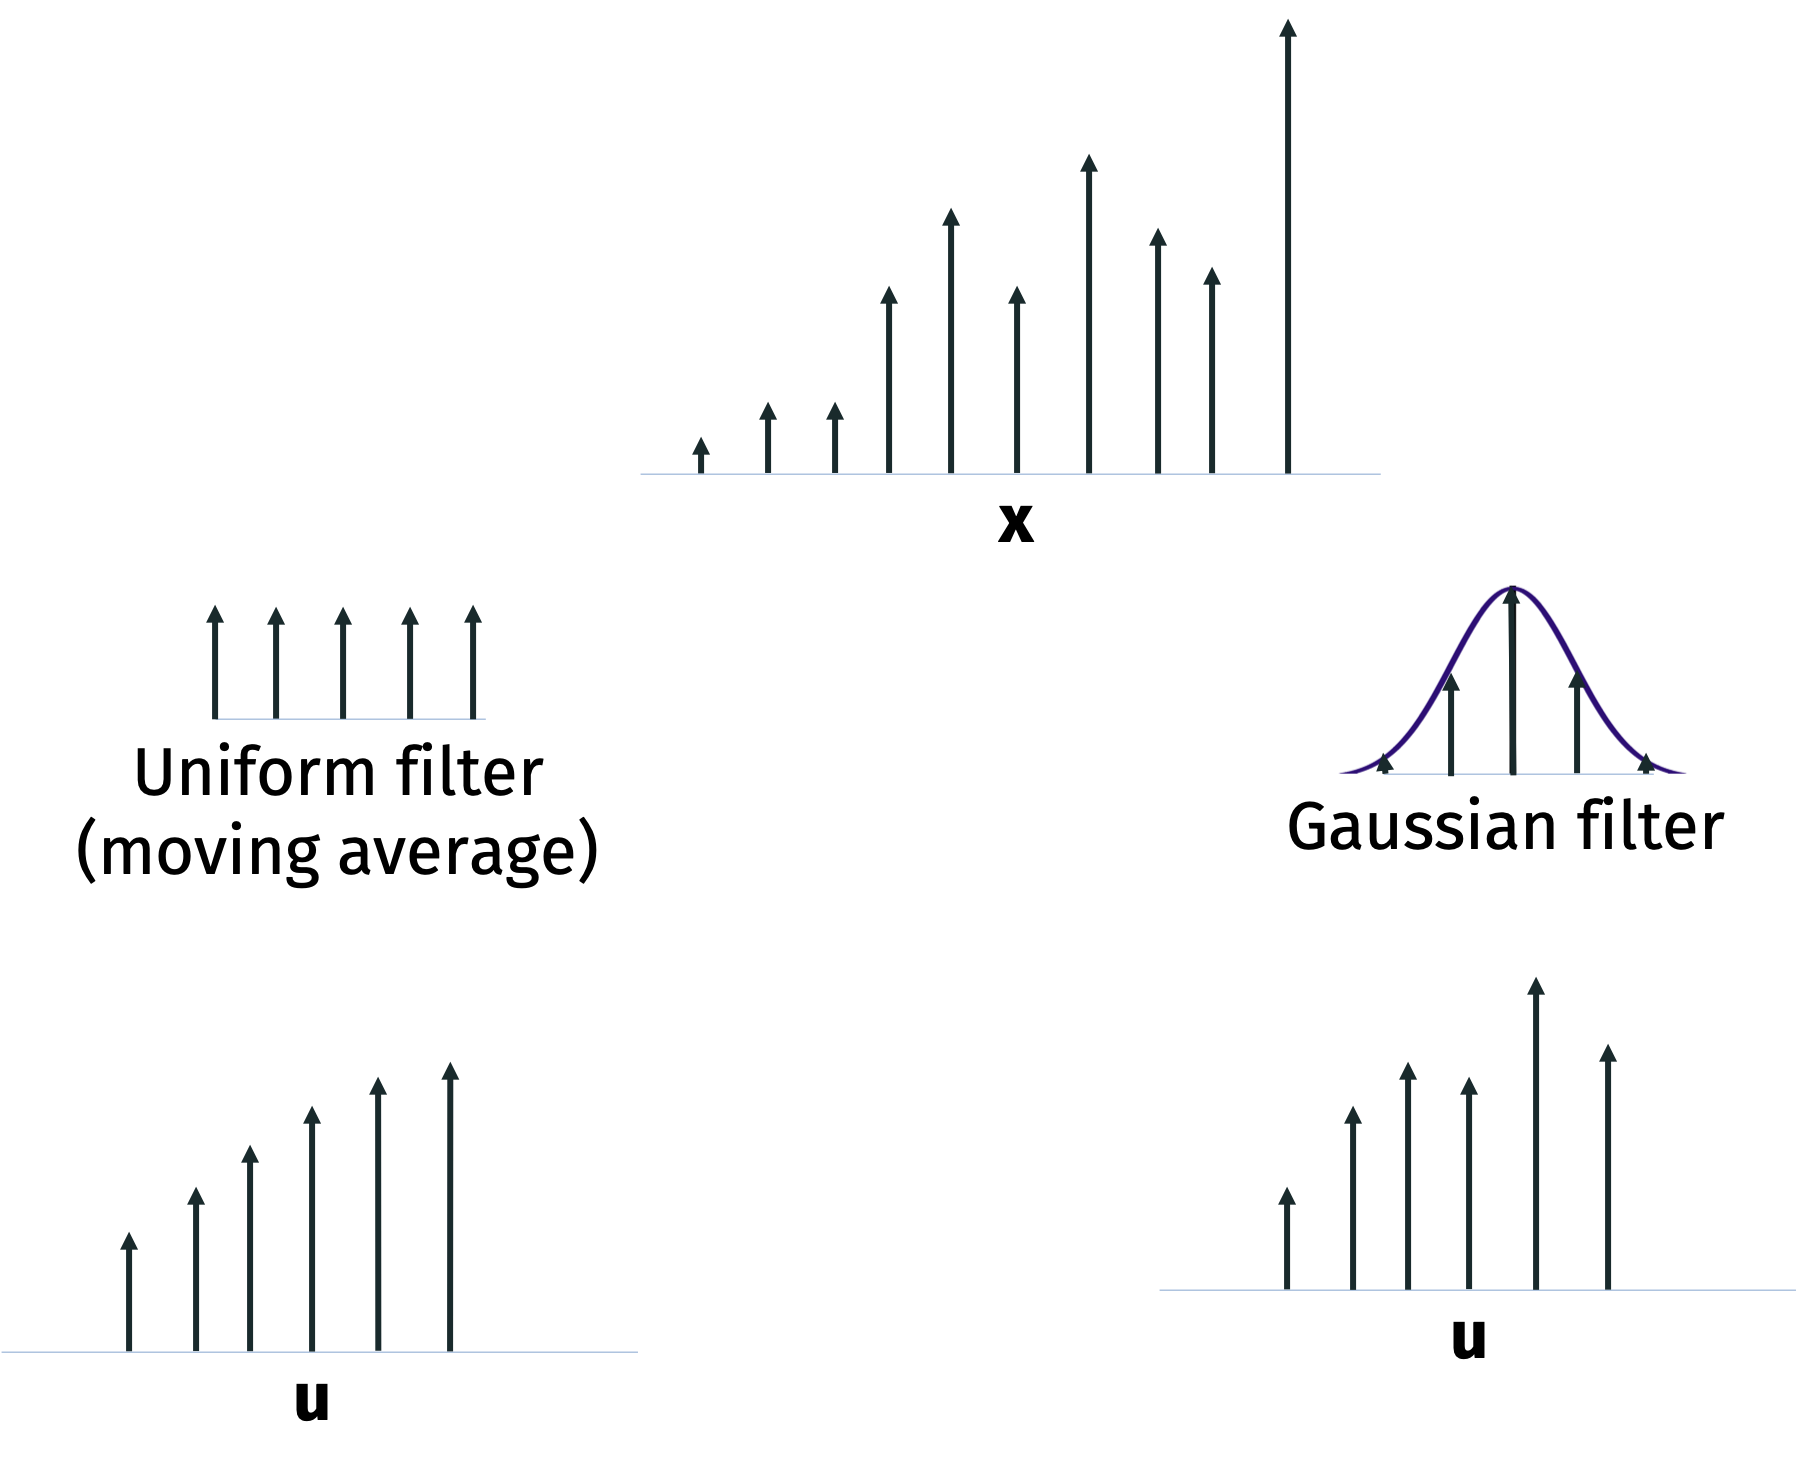
\includegraphics[width=.9\textwidth]{smoothing1d.png}
	\end{center}
	\end{frame}

	\begin{frame}
	\frametitle{smoothing filters}
	Useful for smoothing time-series data, or removing noise/static from audio data. 
	\begin{center}
		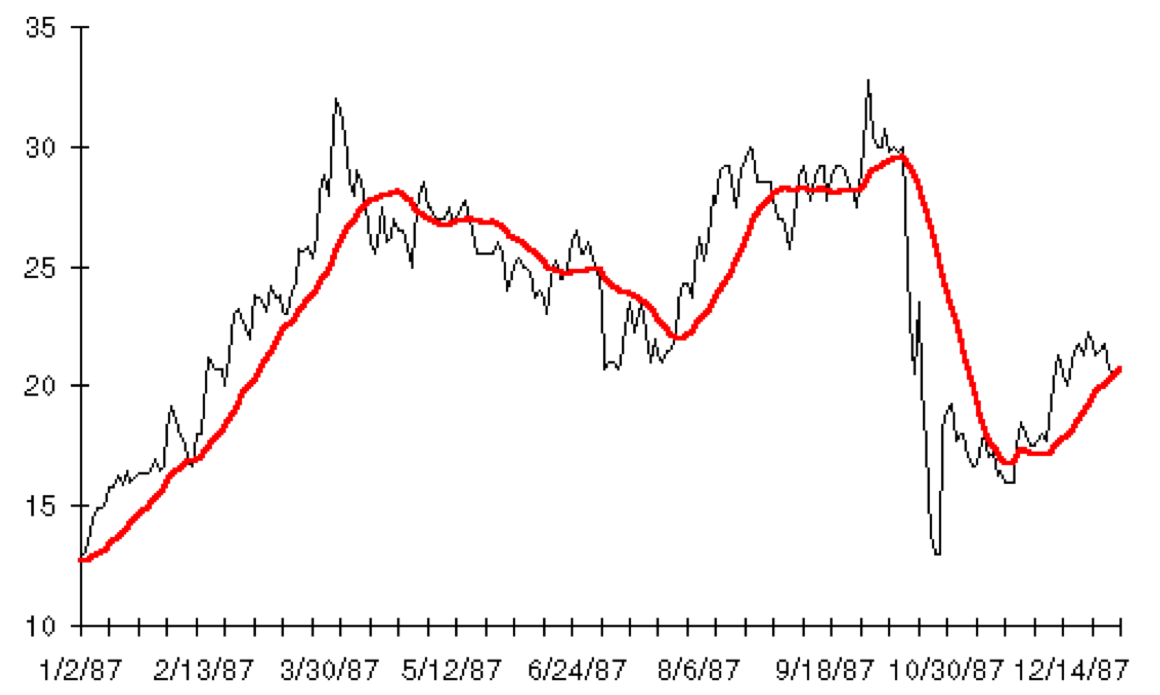
\includegraphics[width=.5\textwidth]{smoothtime_series.png}
	\end{center}
	Replaces every data point with a \emph{local average}.
	\end{frame}

	\begin{frame}
	\frametitle{smoothing in two dimensions}
	In two dimensions:
	\begin{itemize}
		\item Uniform filter: $\bv{w}_{i,j} = \frac{1}{k_1k_2}$ for $i = 1,\ldots, k_1$, $j = 1,\ldots, k_2$.
		\item Gaussian filter: $\vec{w}_i \sim \exp^{\frac{(i-k_1/2)^2 + (j-k_2/2)^2}{\sigma^2}}$ for $i = 1,\ldots, k_1$, $j = 1,\ldots, k_2$.
	\end{itemize}
\begin{center}
	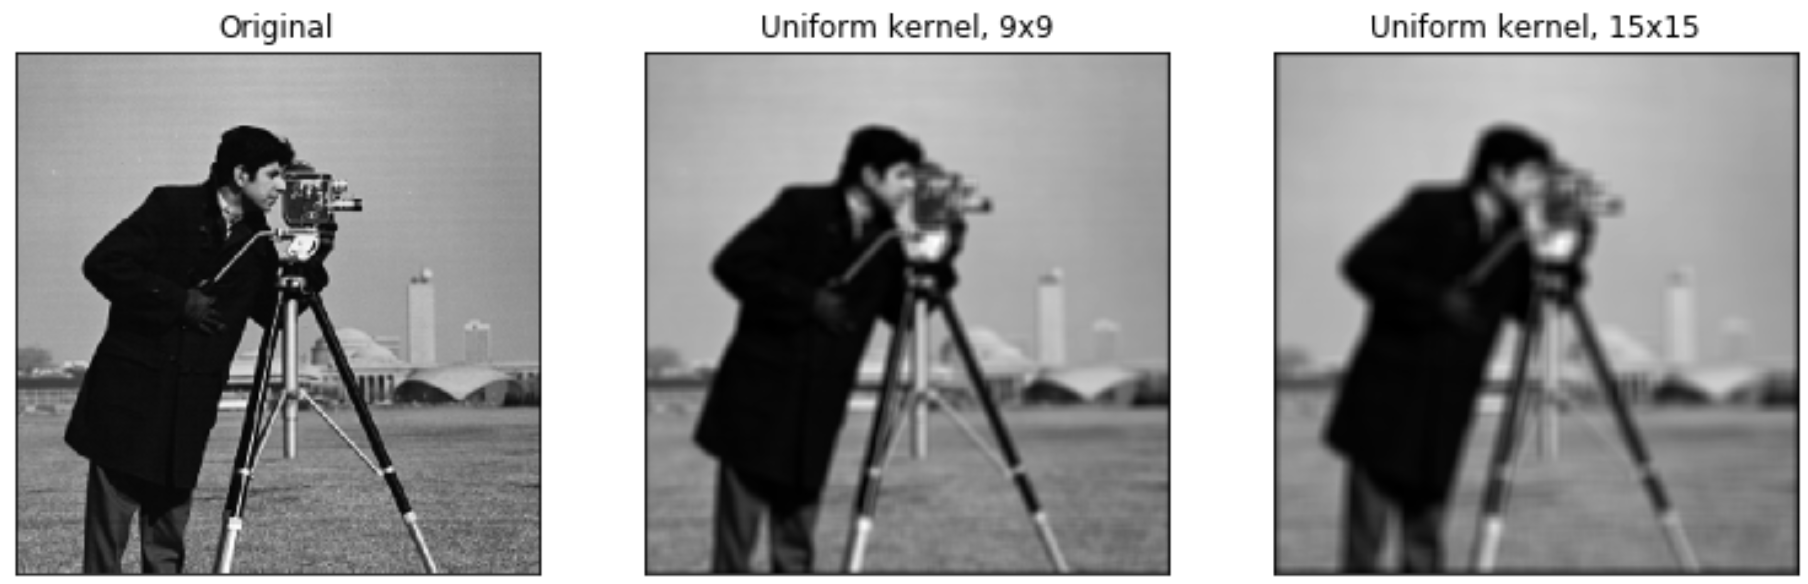
\includegraphics[width=.8\textwidth]{uniform.png}
	
	Larger filter equates to more smoothing. 
\end{center}
	\end{frame}

\begin{frame}
	\frametitle{smoothing in two dimensions}
	For Gaussian filter, you typically choose $k \gtrsim 2\sigma$ to capture the fall-off of the Gaussian. 
	\begin{center}
		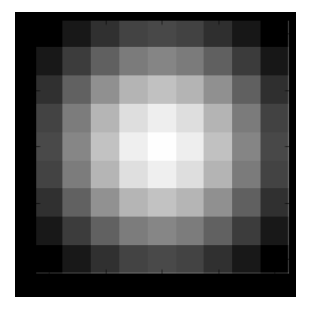
\includegraphics[width=.2\textwidth]{gaussian_filter.png}
		
		
		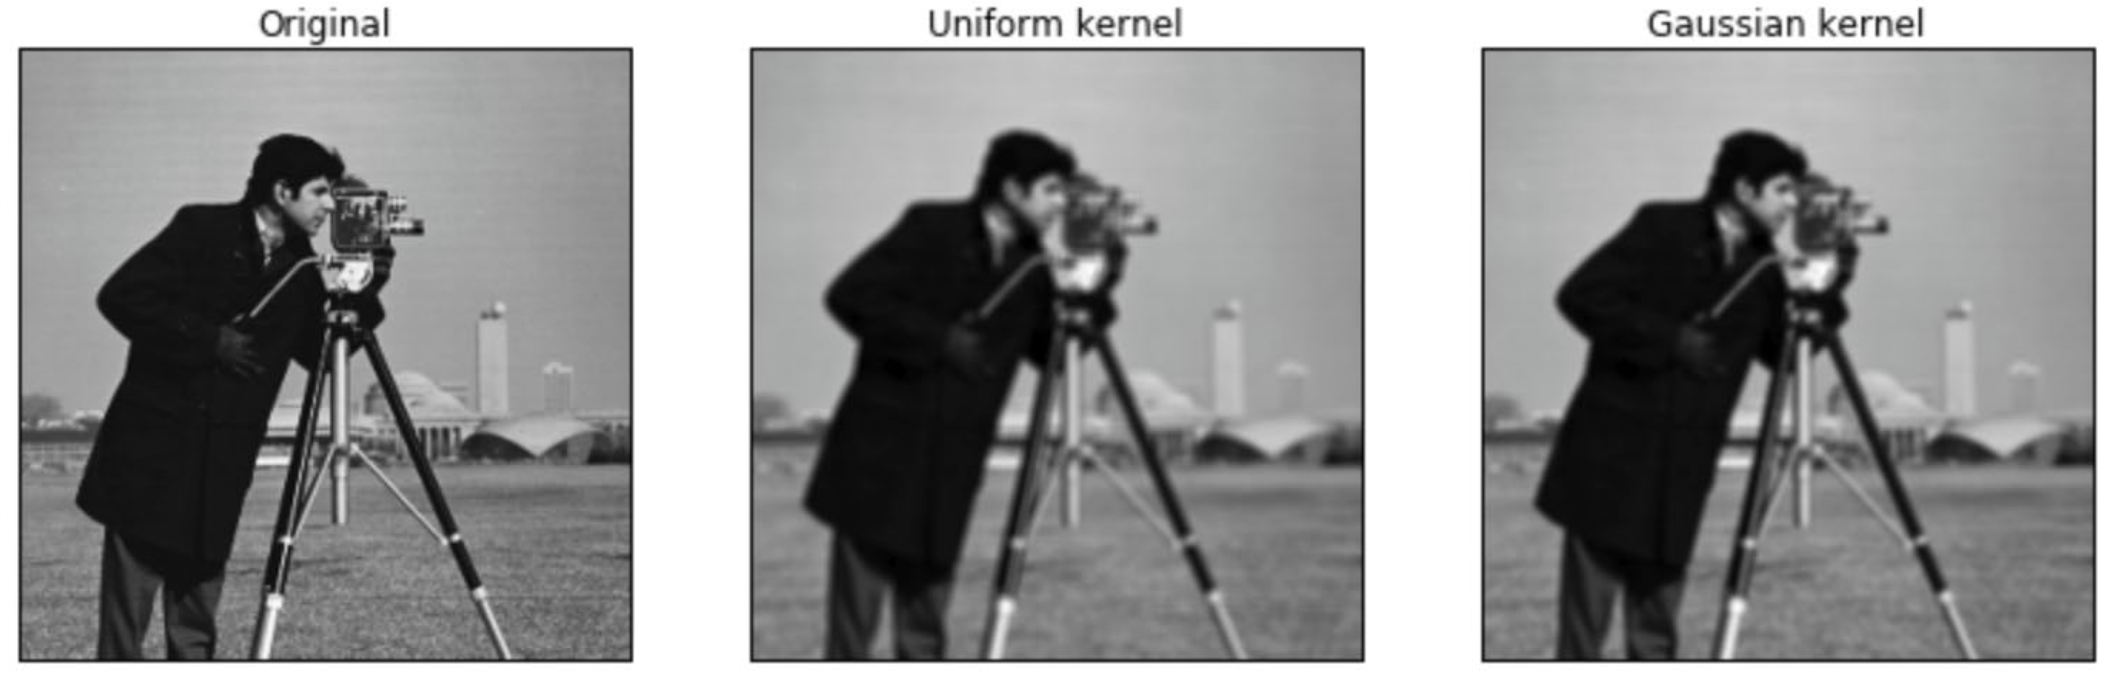
\includegraphics[width=.8\textwidth]{uniform_vs_gauss.png}
	\end{center}

	Both approaches effectively denoise and smooth images. 
\end{frame}

	\begin{frame}
	\frametitle{smoothing for feature extraction}
	When combined with other feature extractors, smoothing at various levels allows the algorithm to focus on high-level features over low-level features.
	\begin{center}
		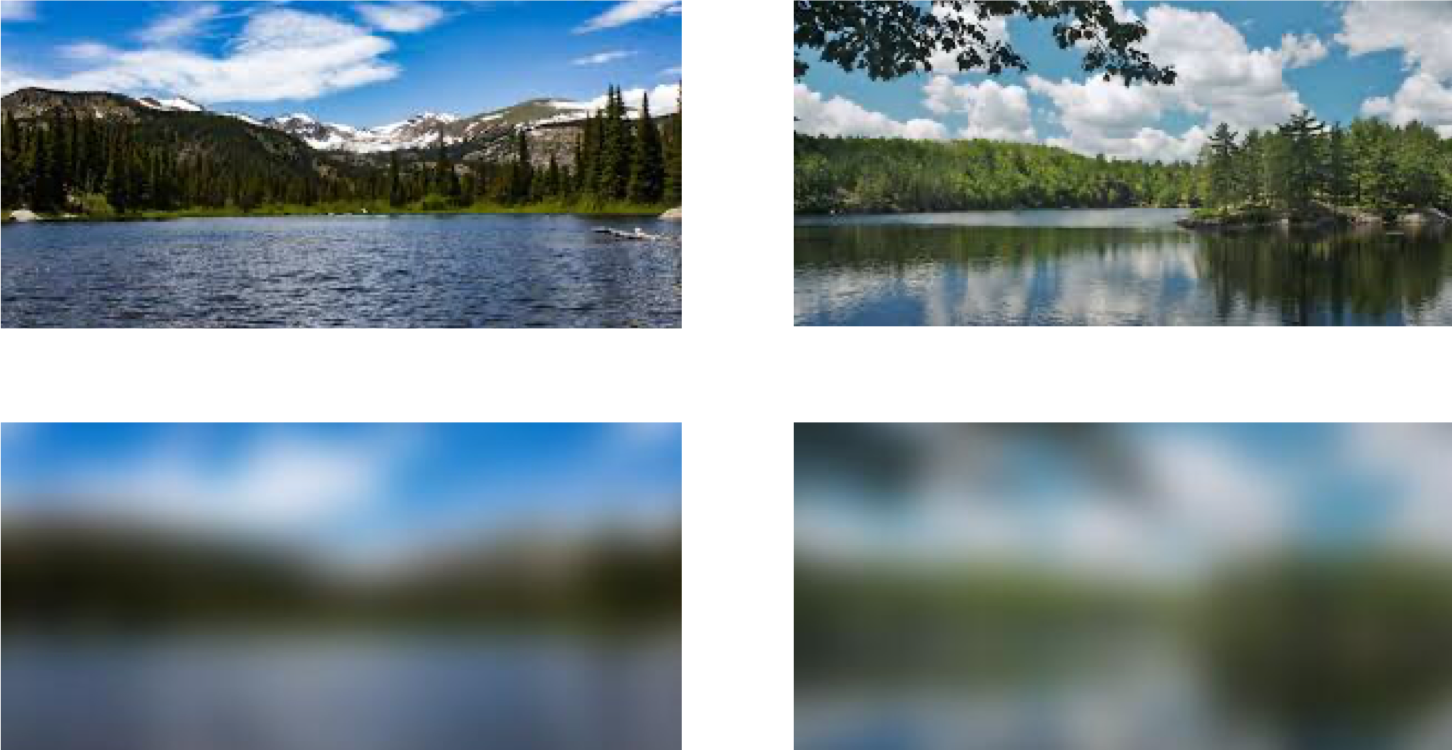
\includegraphics[width=.9\textwidth]{blurred_compare.png}
	\end{center}
	\end{frame}

	\begin{frame}
	\frametitle{applications of convolution}
	\textbf{Application 2:} Pattern matching.
	
Slide a pattern over an image. Output of convolution will be \emph{higher} when pattern \emph{correlates well} with underlying image.
	\begin{center}
	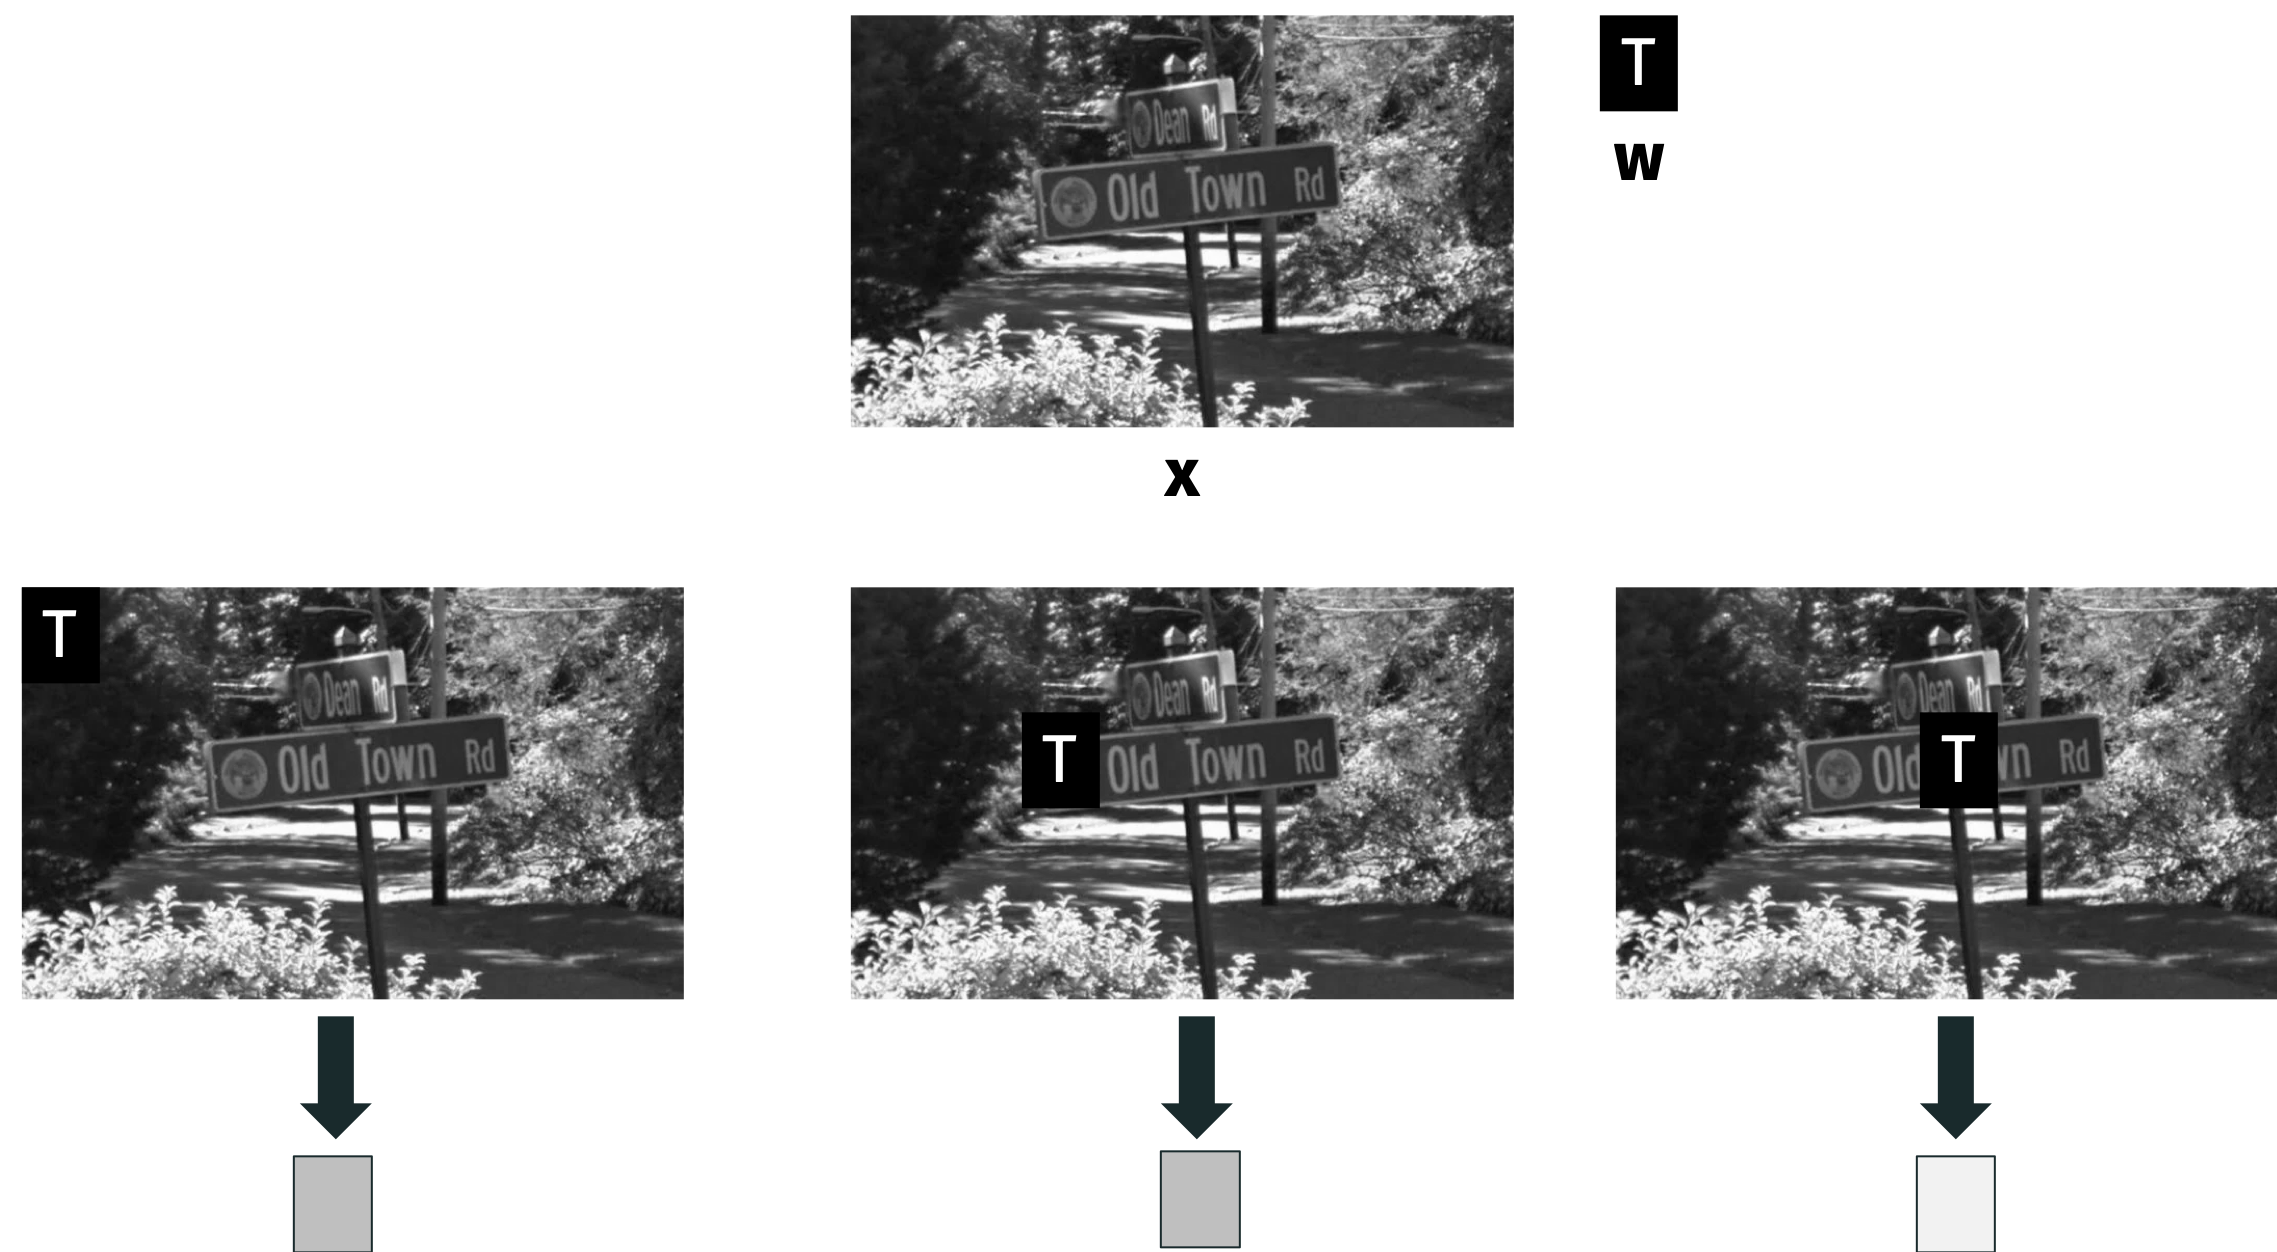
\includegraphics[width=.9\textwidth]{matched_filter.png}
	\end{center}
	\end{frame}

	\begin{frame}
	\frametitle{local pattern matching}
	\textbf{Applications of local pattern matching}:
	\begin{itemize}
	\item Check if an image contains text.
	\item Look for specific sound in audio recording.
	\item Check for other well-structured objects
	\end{itemize}
	
	\end{frame}

	\begin{frame}
	\frametitle{3d convolution}
	Recall that \emph{color images} actually have three color channels for \textbf{red}, \textbf{green}, \textbf{blue}s. Each pixel is represented by 3 values (e.g. in $0,\ldots, 255$) giving the intensity in each channel. 
	
	$[0,0,0]$ = black, $[0,0,0]$ = white, $[1,0,0]$ = pure red, etc.
	
	\textbf{View image as 3D \alert{tensor}}:
	\vspace{-1em}
	\begin{center}
			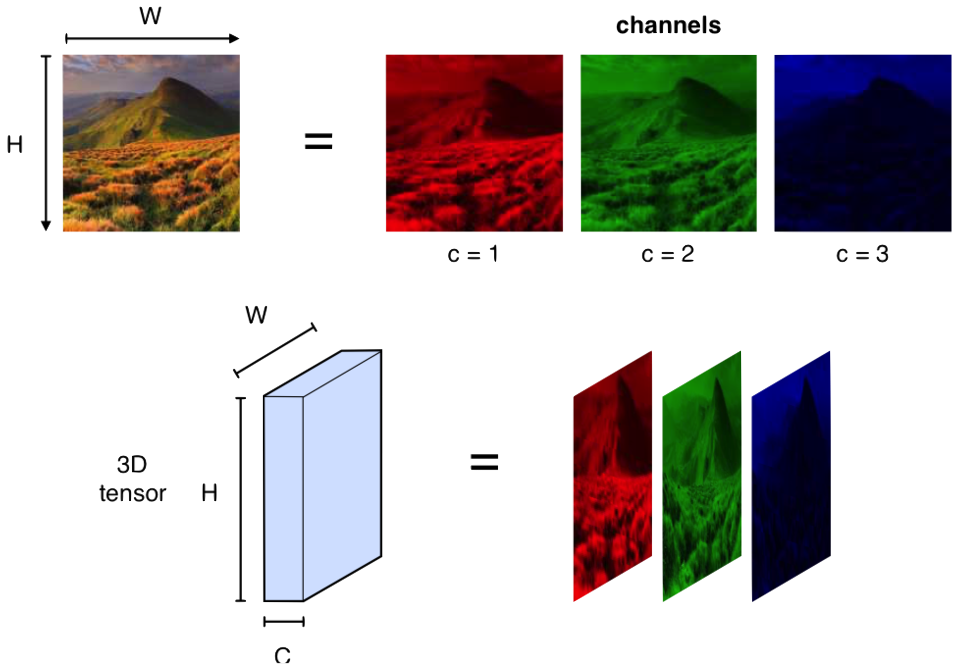
\includegraphics[width=.6\textwidth]{image_tensor.png}
	\end{center}
	
	\end{frame}

	\begin{frame}
	\frametitle{3d convolution}
	Can be convolved with 3D filter:
				\small
	\begin{definition}[Discrete 2D convolution]
		Given tensors $\bv{x} \in \R^{d_1\times d_2 \times d_3}$ and $\bv{w} \in \R^{k_1\times k_2 \times k_3}$ the discrete convolution $\bv{x}\circledast \bv{w}$ is a $(d_1 - k_1 + 1)\times (d_2 - k_2 + 1) \times (d_3 - k_3 + 1)$ tensor with:
		\vspace{-1em}
		\begin{align*}
		[\bv{x}\circledast \bv{w}]_{i,j,g} = \sum_{\ell=1}^{k_1}\sum_{m=1}^{k_2}\sum_{n=1}^{k_3} \bv{x}_{(i + \ell -1),(j + m -1),(g + n -1)}\cdot \bv{w}_{\ell,m,n}
		\end{align*}
		\vspace{-1em}
	\end{definition}
	\begin{center}
	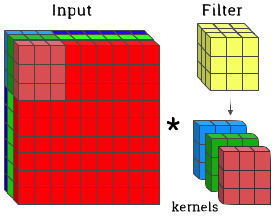
\includegraphics[width=.5\textwidth]{tensor.png}
	\end{center}
	
	\end{frame}

	\begin{frame}
	\frametitle{3d convolution}
	\begin{center}
	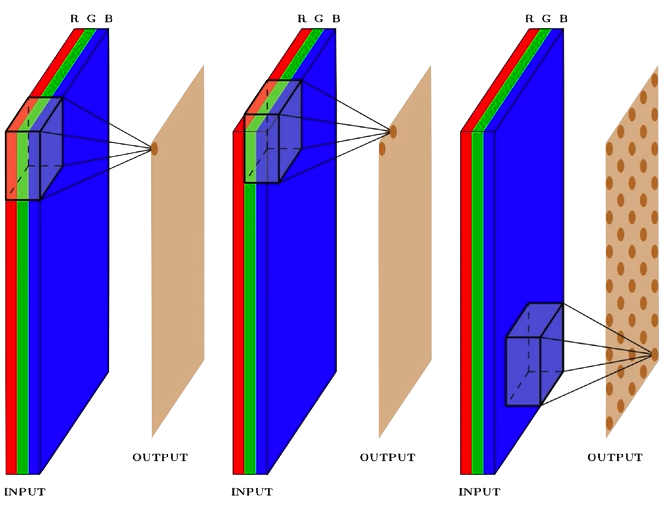
\includegraphics[width=.7\textwidth]{3dconov.png}
	\end{center}
	\end{frame}


\begin{frame}
	\frametitle{3d convolution}
	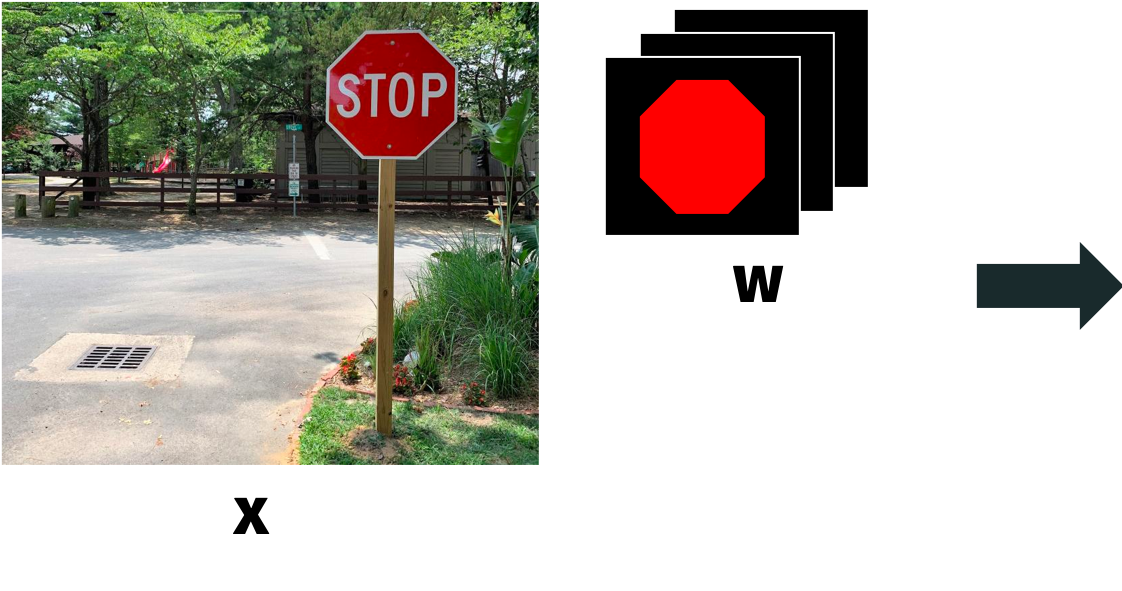
\includegraphics[width=.6\textwidth]{stop_convolve.png}
	
	\begin{center}
		Relatively robust to imperfections, damage, occlusion, etc.
		
		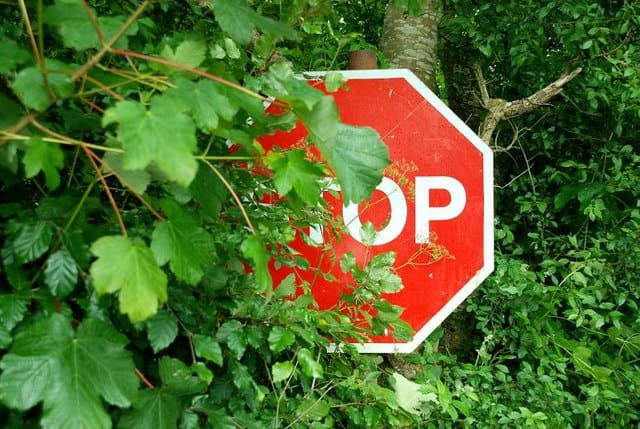
\includegraphics[width=.3\textwidth]{hidden_stop.jpg} 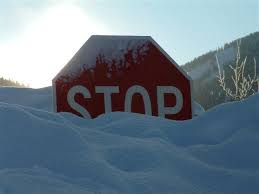
\includegraphics[width=.3\textwidth]{hiddenstop_2.jpeg}
		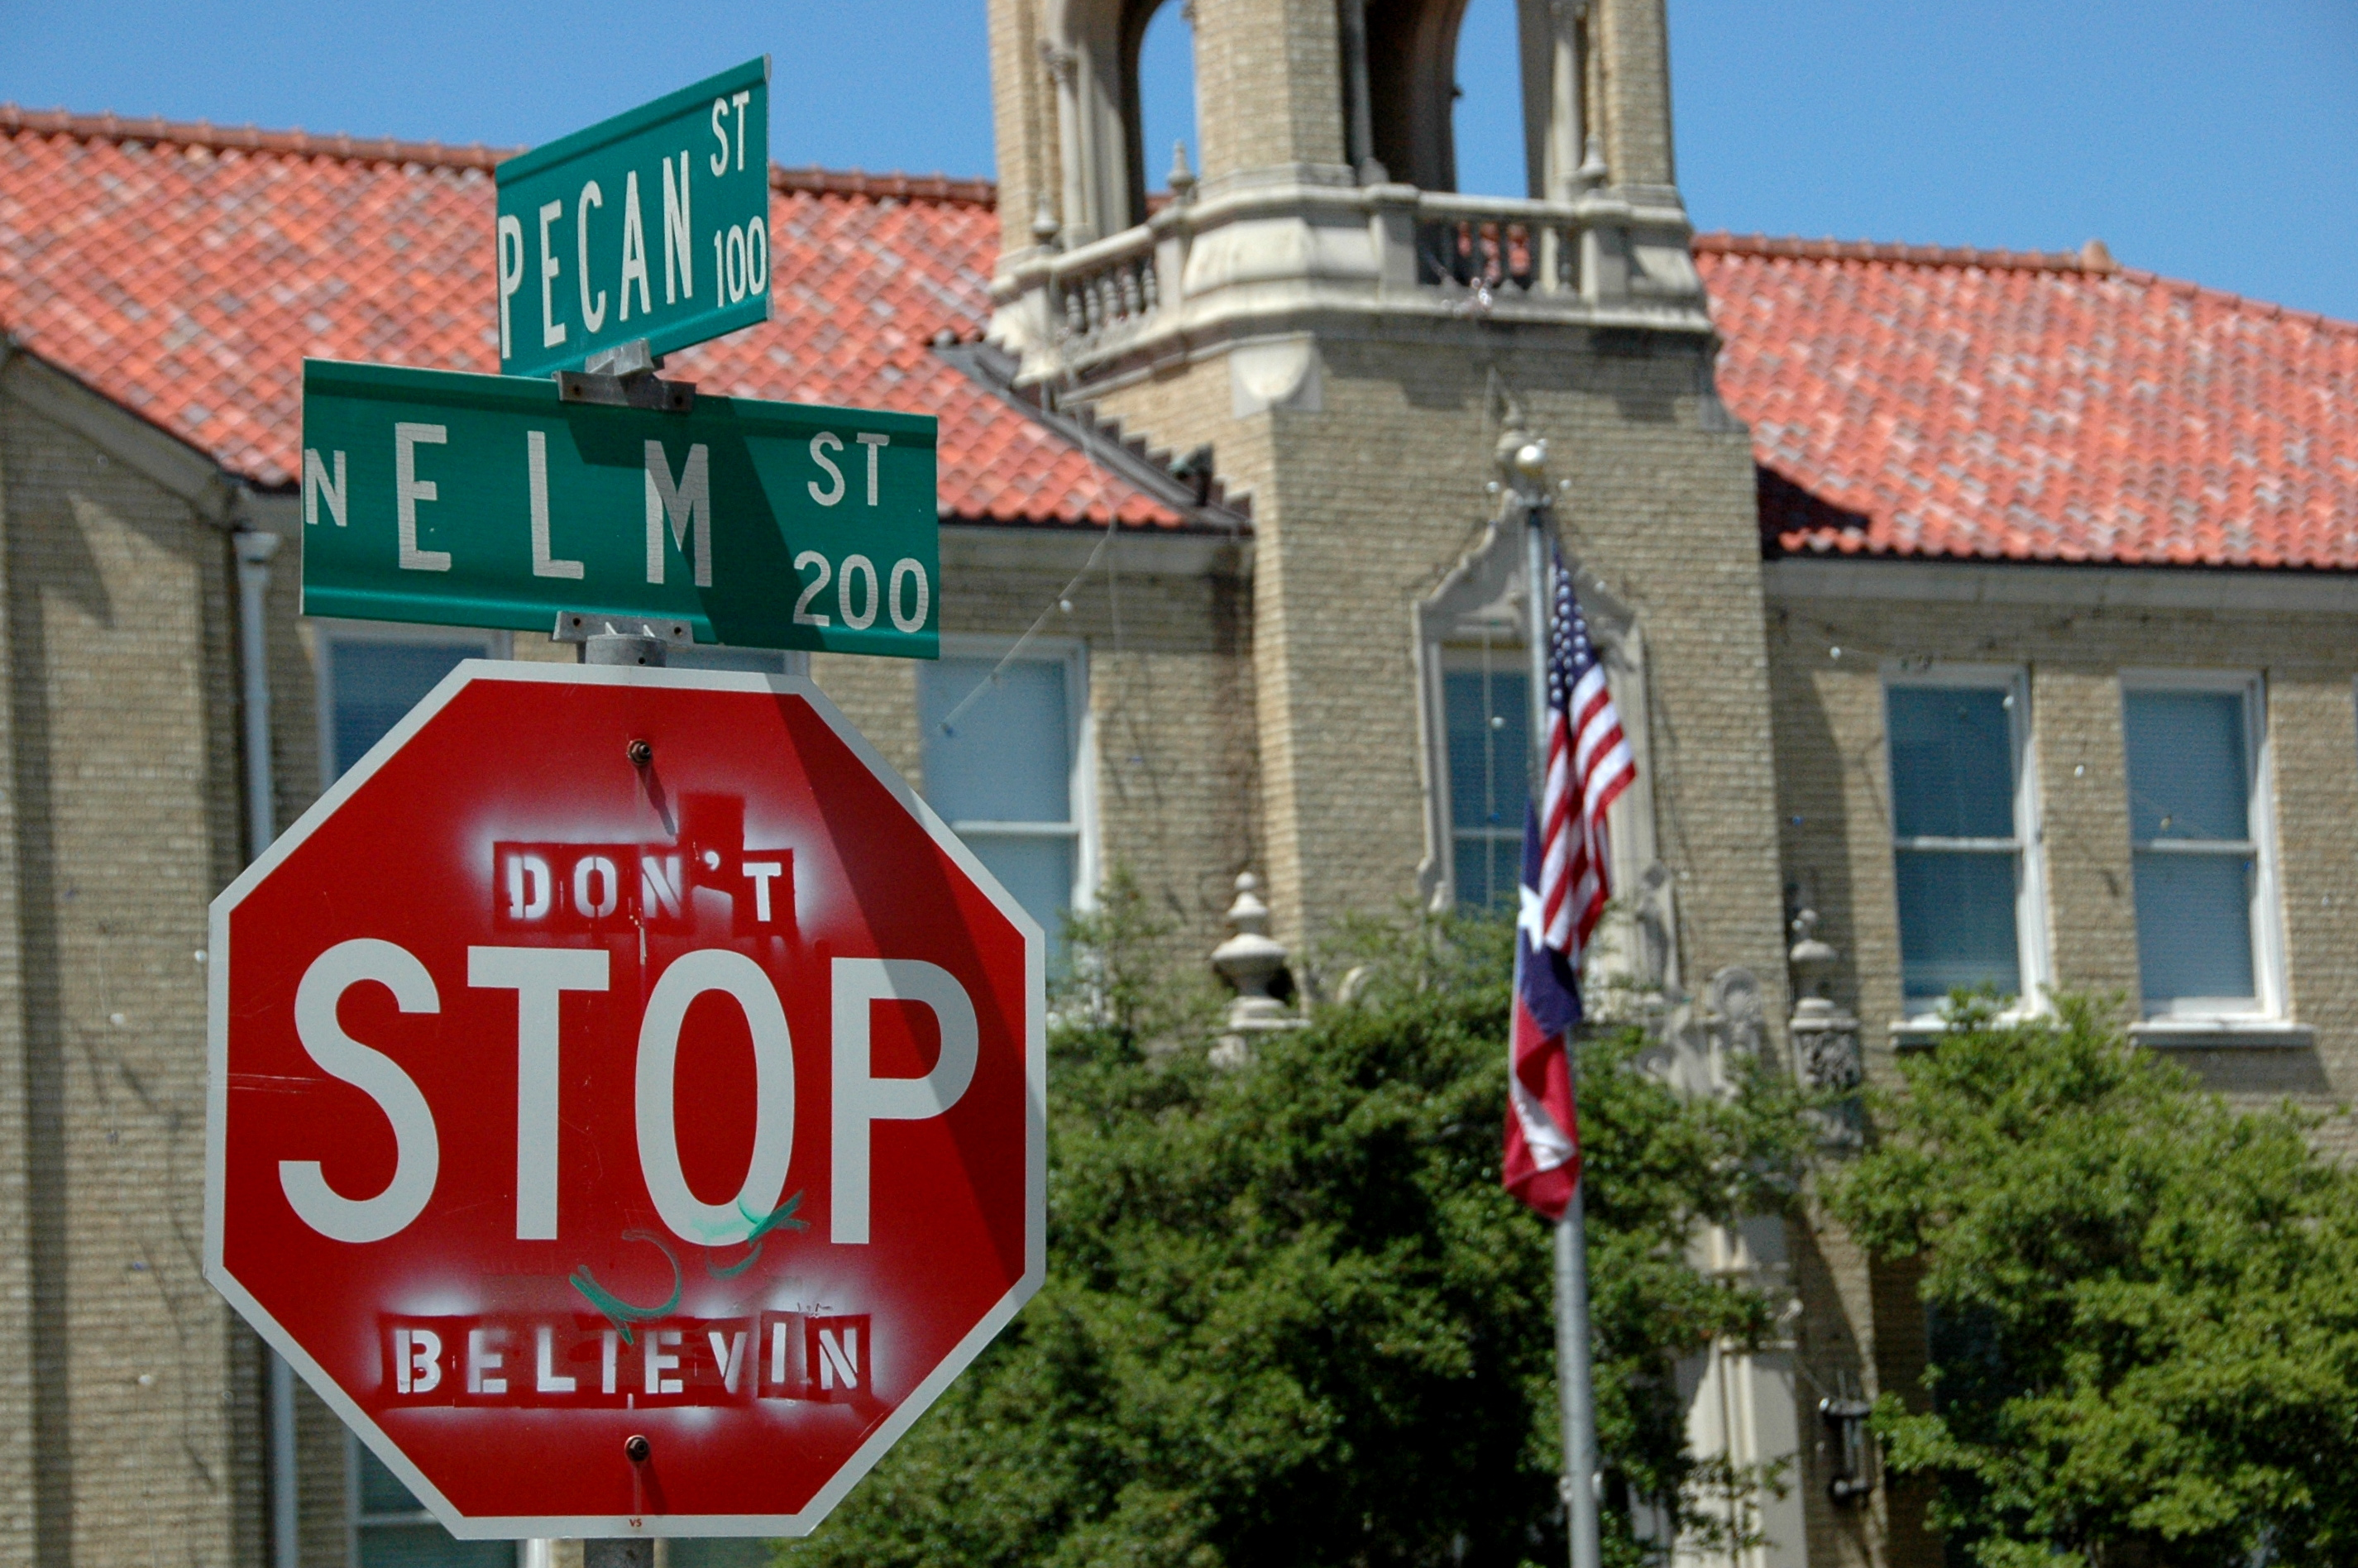
\includegraphics[width=.3\textwidth]{stopsign_3.jpg}
	\end{center}	
\end{frame}

\begin{frame}
	\frametitle{3d convolution}
	In general extracting different color information is very useful for image understanding:
	\begin{center}
		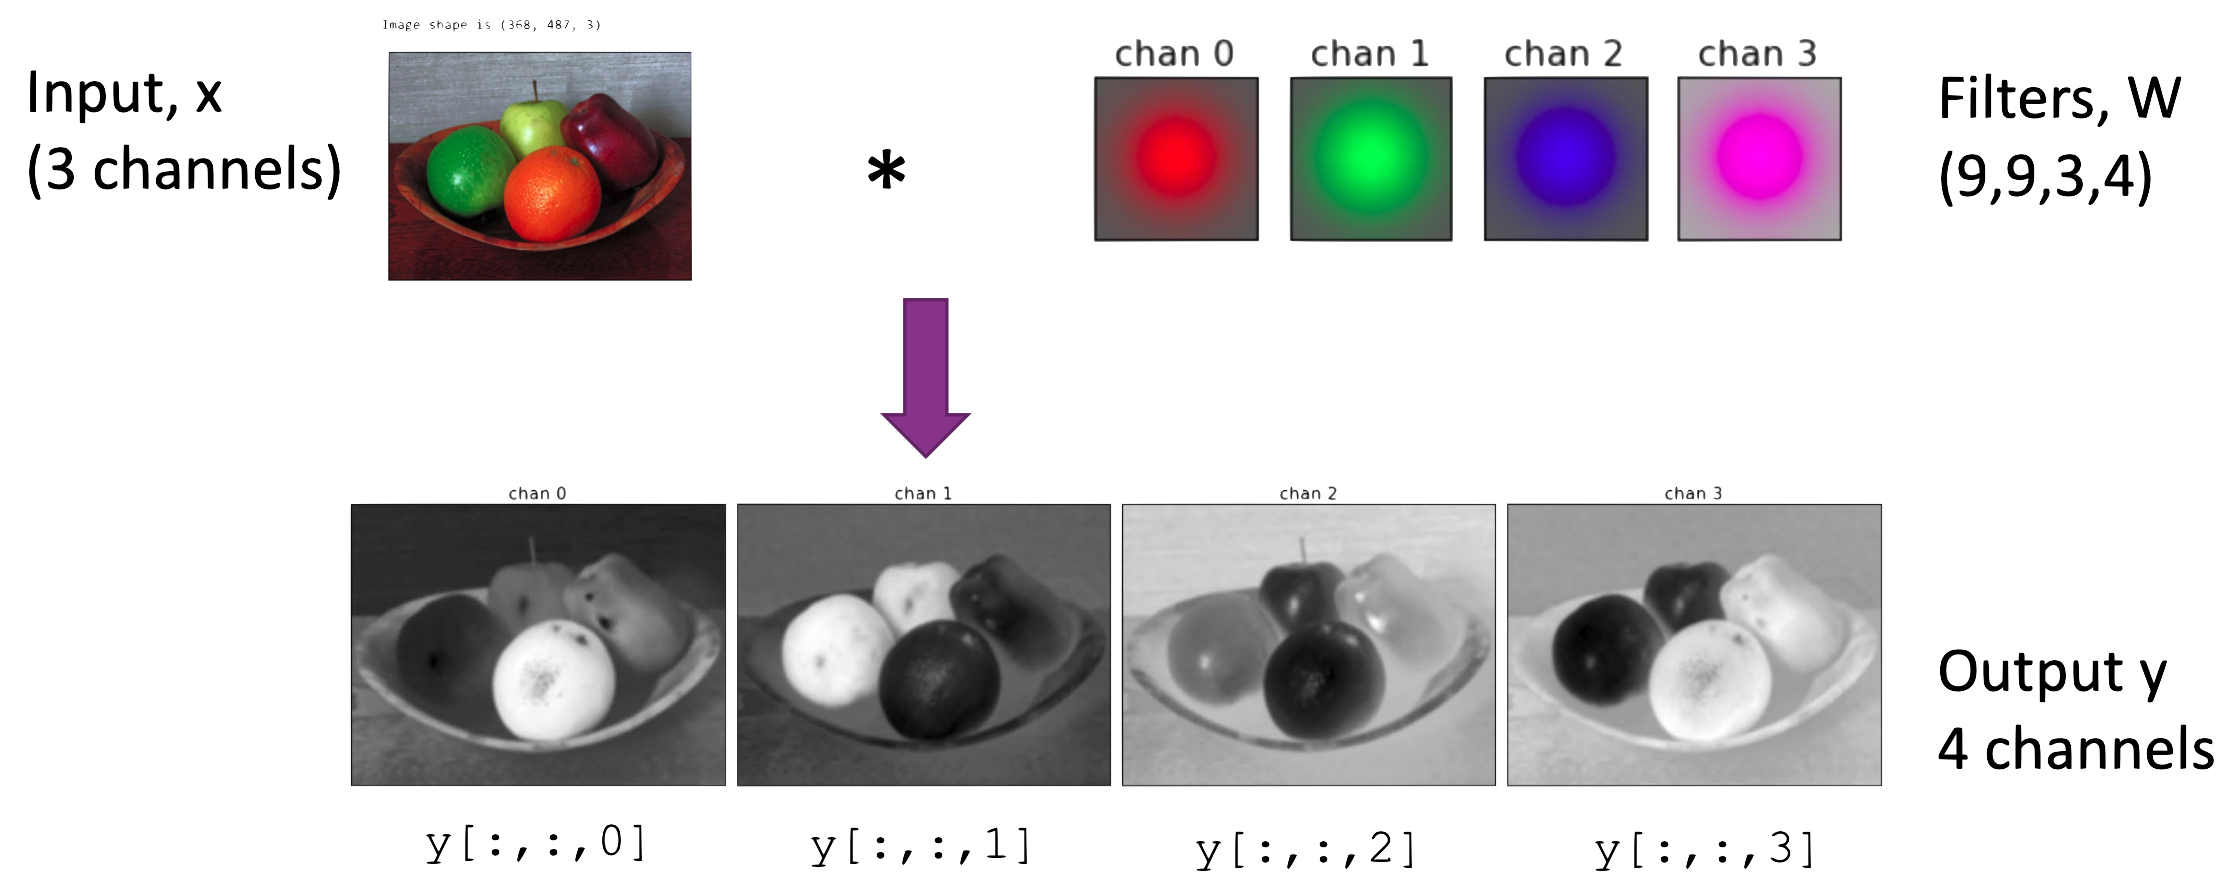
\includegraphics[width=\textwidth]{color_extract.png}
	\end{center}	
\end{frame}

\begin{frame}
	\frametitle{frequency detection}
	\textbf{Less obvious example of pattern matching:} Frequency detection in audio.
	\begin{center}
		Any 1D signal (including a sound wave) can be decomposed into component frequencies:
		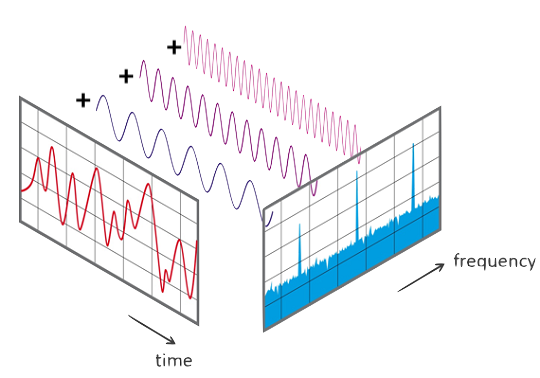
\includegraphics[width=.6\textwidth]{simpledft.png}
		
		$\vec{x}(t) = \sin(f_1t + s_1) + \sin(f_2t + s_2) + \sin(f_3t + s_3) + \ldots$
	\end{center}
\end{frame}

\begin{frame}
	\frametitle{frequency detection}
	\small
	Convolve audio signal with snippet of pure frequency to determine where difference frequencies are prevalent. Detect things like:
	\begin{itemize}
		\item Common notes in a song.
		\item Different instruments. 
		\item Human voices vs. other noise.
	\end{itemize}
	\begin{center}
		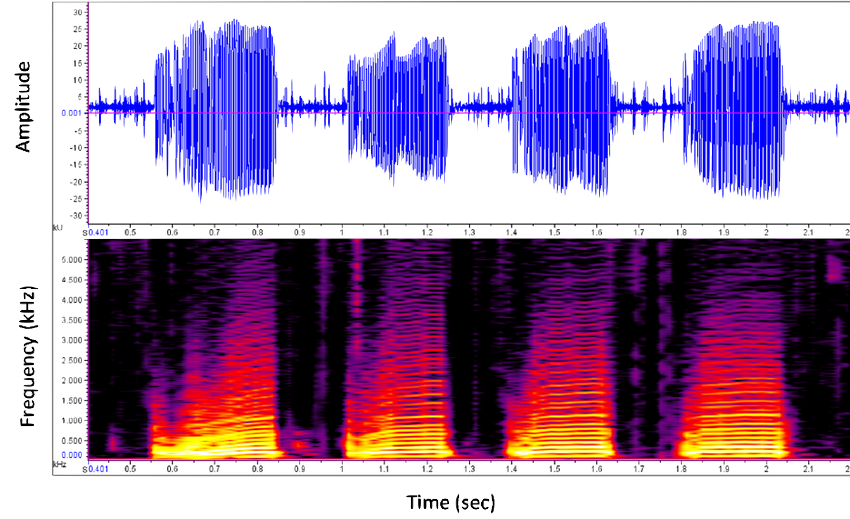
\includegraphics[width=.5\textwidth]{spectrogram.png}
		
		Main idea behind short-time Fourier transforms/spectrograms.
	\end{center}
\end{frame}

	\begin{frame}
	\frametitle{applications of convolution}
	\small
	\textbf{Application 3:} Edge detection.
	
	Consider a 2d \emph{Sobel filter:}
	\begin{align*}
	W_1 &= \begin{bmatrix}
	1 & 0 & -1\\
	2 & 0 & -2\\
	1 & 0 & -1
	\end{bmatrix} & 	
	W_2 &= \begin{bmatrix}
	1 & 2 & 1\\
	0 & 0 & 0\\
	-1 & -2 & -1
	\end{bmatrix}
	\end{align*}
	\begin{center}
		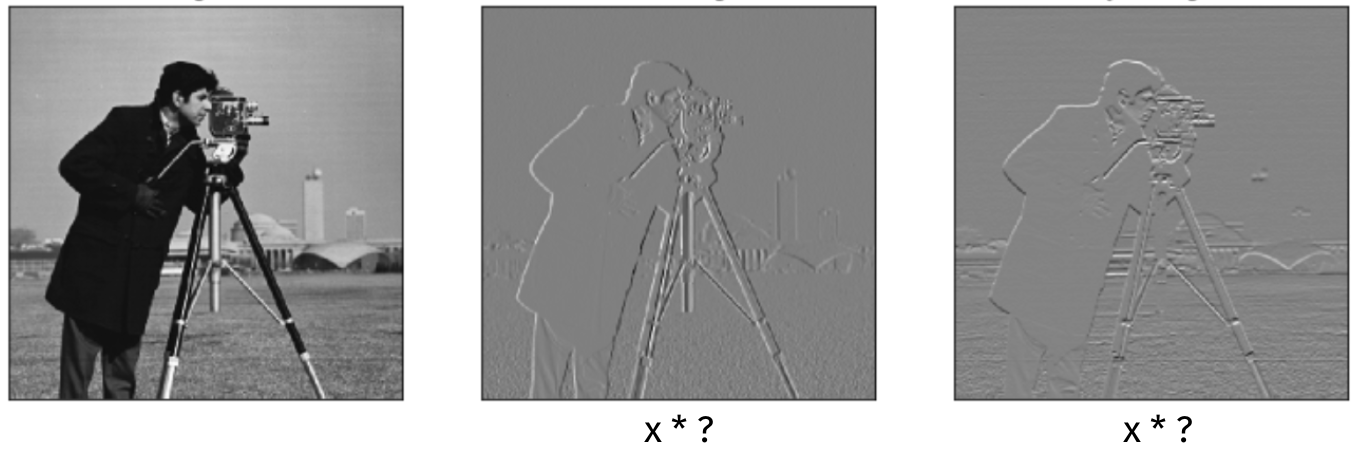
\includegraphics[width=\textwidth]{conv_test.png}
	\end{center}
\end{frame}

	\begin{frame}
	\frametitle{applications of convolution}
	Edges with different orientations are \emph{low-level} features compared to what we might get from e.g. explicit pattern matching. They still provide some immediately useful information about an image.
	\begin{center}
		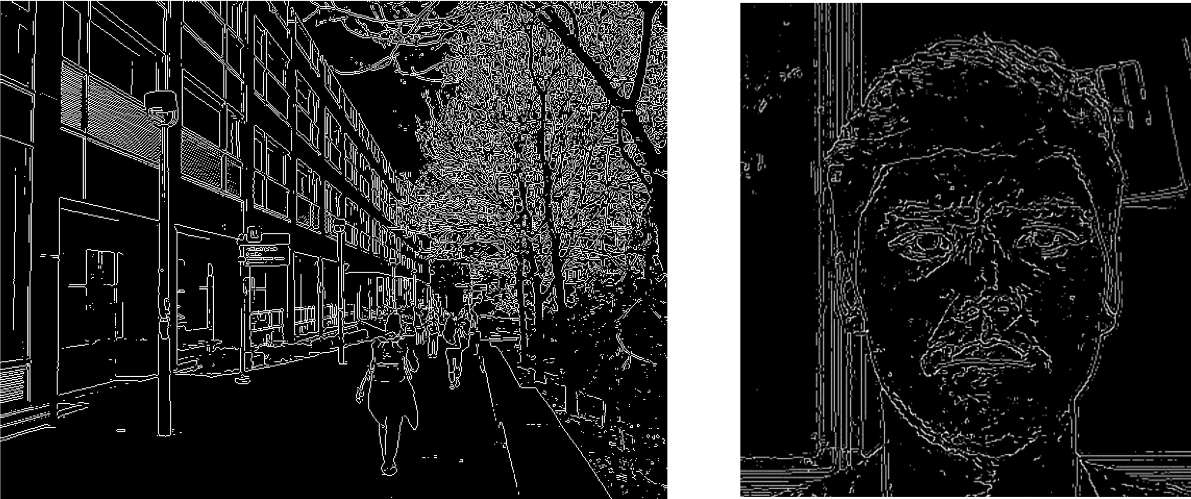
\includegraphics[width=.5\textwidth]{edge_hint.png}
	\end{center}
More useful when \emph{combined} to build higher-level features.
	
I 	\end{frame}

	\begin{frame}
	\frametitle{applications of convolution}
	\textbf{Next class:} 
	Design neural network architectures that have convolutionoal operations \emph{built-in}. The exact weights are left as free variables. Lowest layers do low-level feature extraction like edge detection, higher layers learn higher-level concepts.
	\begin{center}
		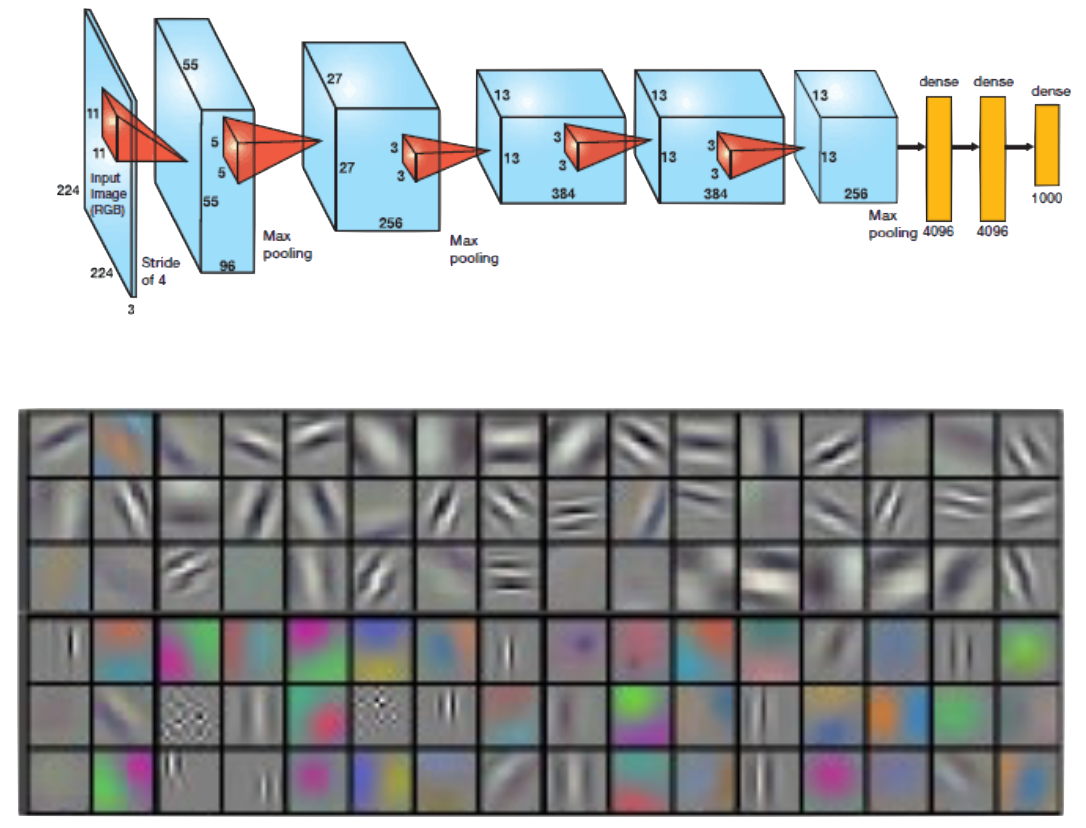
\includegraphics[width=.5\textwidth]{edge_detect.png}
	\end{center}
	
	\end{frame}

\end{document} 



